%%____________________________________________________________________________||
\section{Trigger strategy}
\label{app:triggers}

\begin{figure}[h!]
  \begin{center}
    \subfigure[$200 < \scalht < 400$]{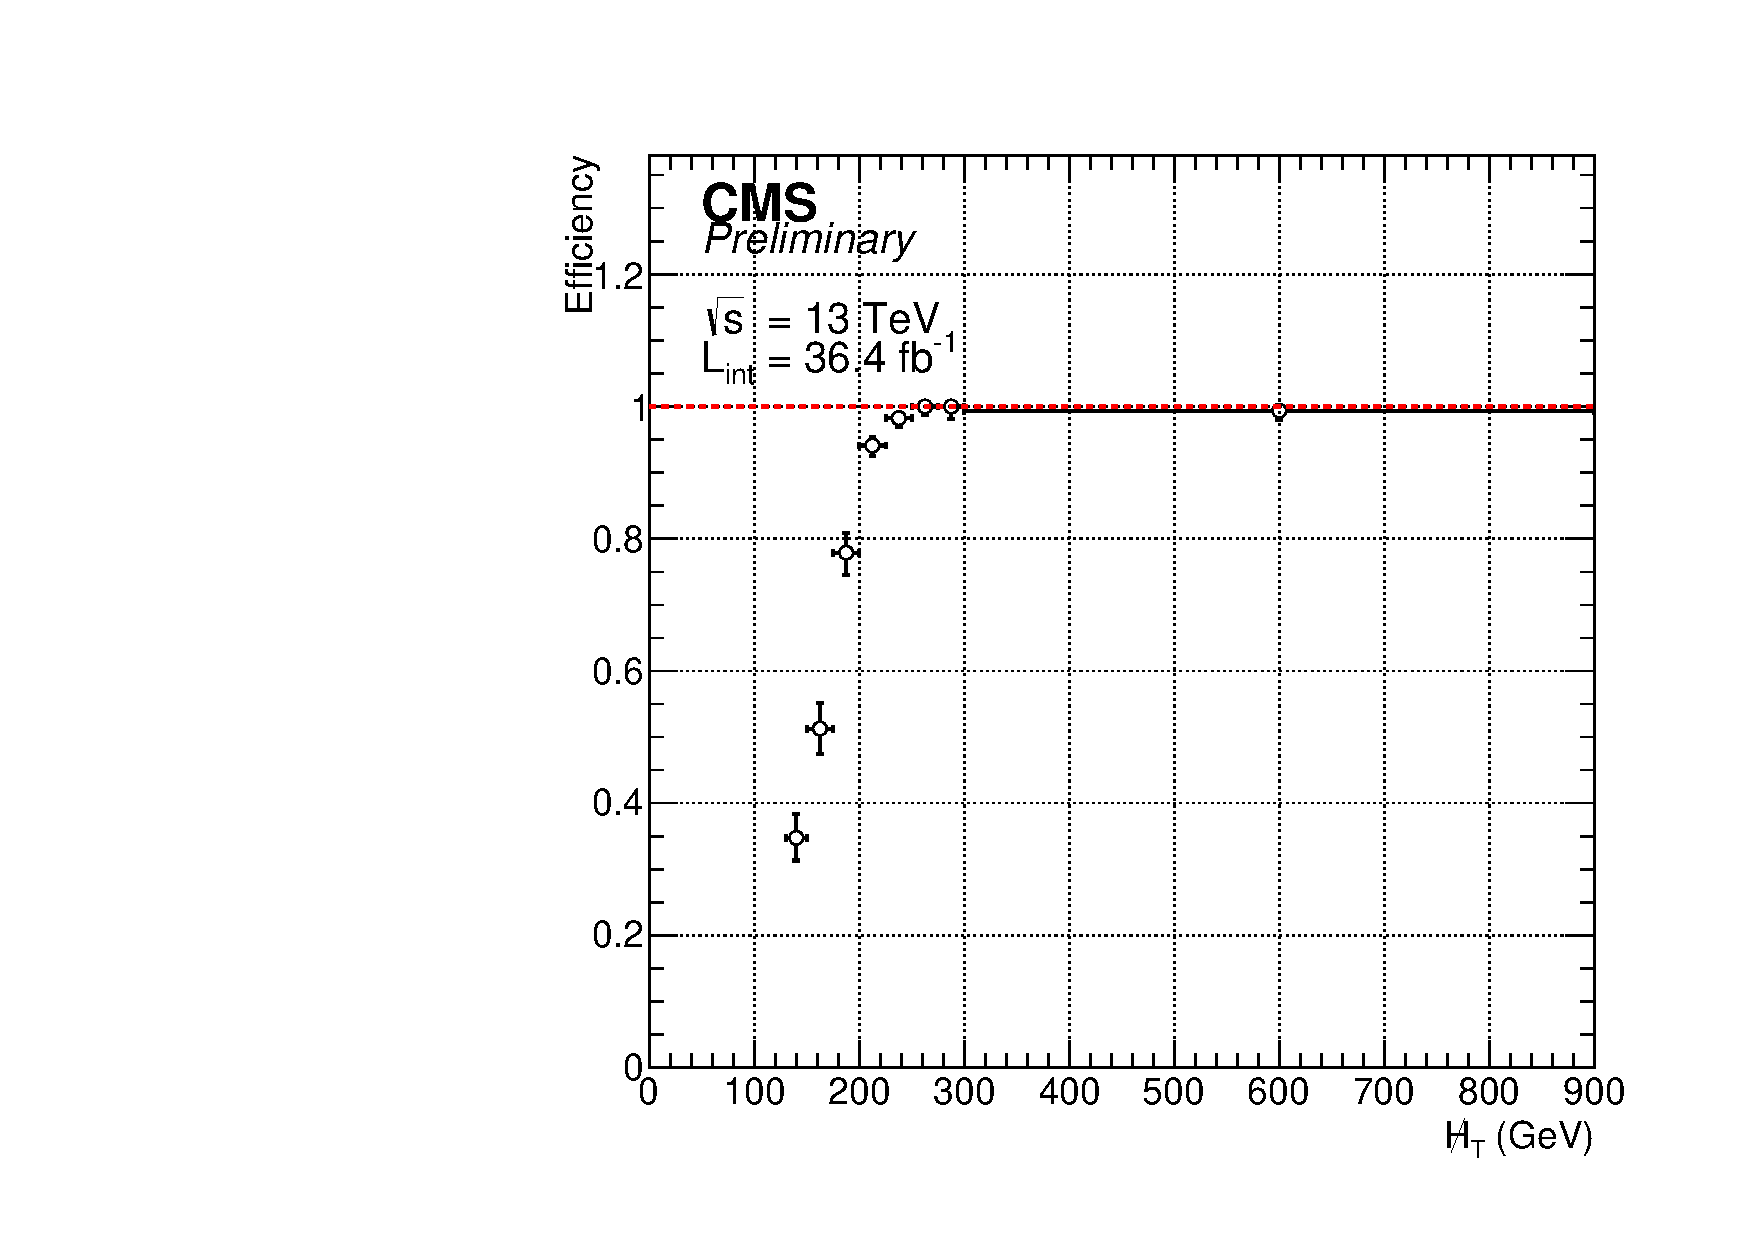
\includegraphics[width=0.28\textwidth]{figures/Trigger/Ele/HLT_AlphaTHT800MonoAll_MoM_all_200to400_mht}} ~
    \subfigure[$200 < \scalht < 400$]{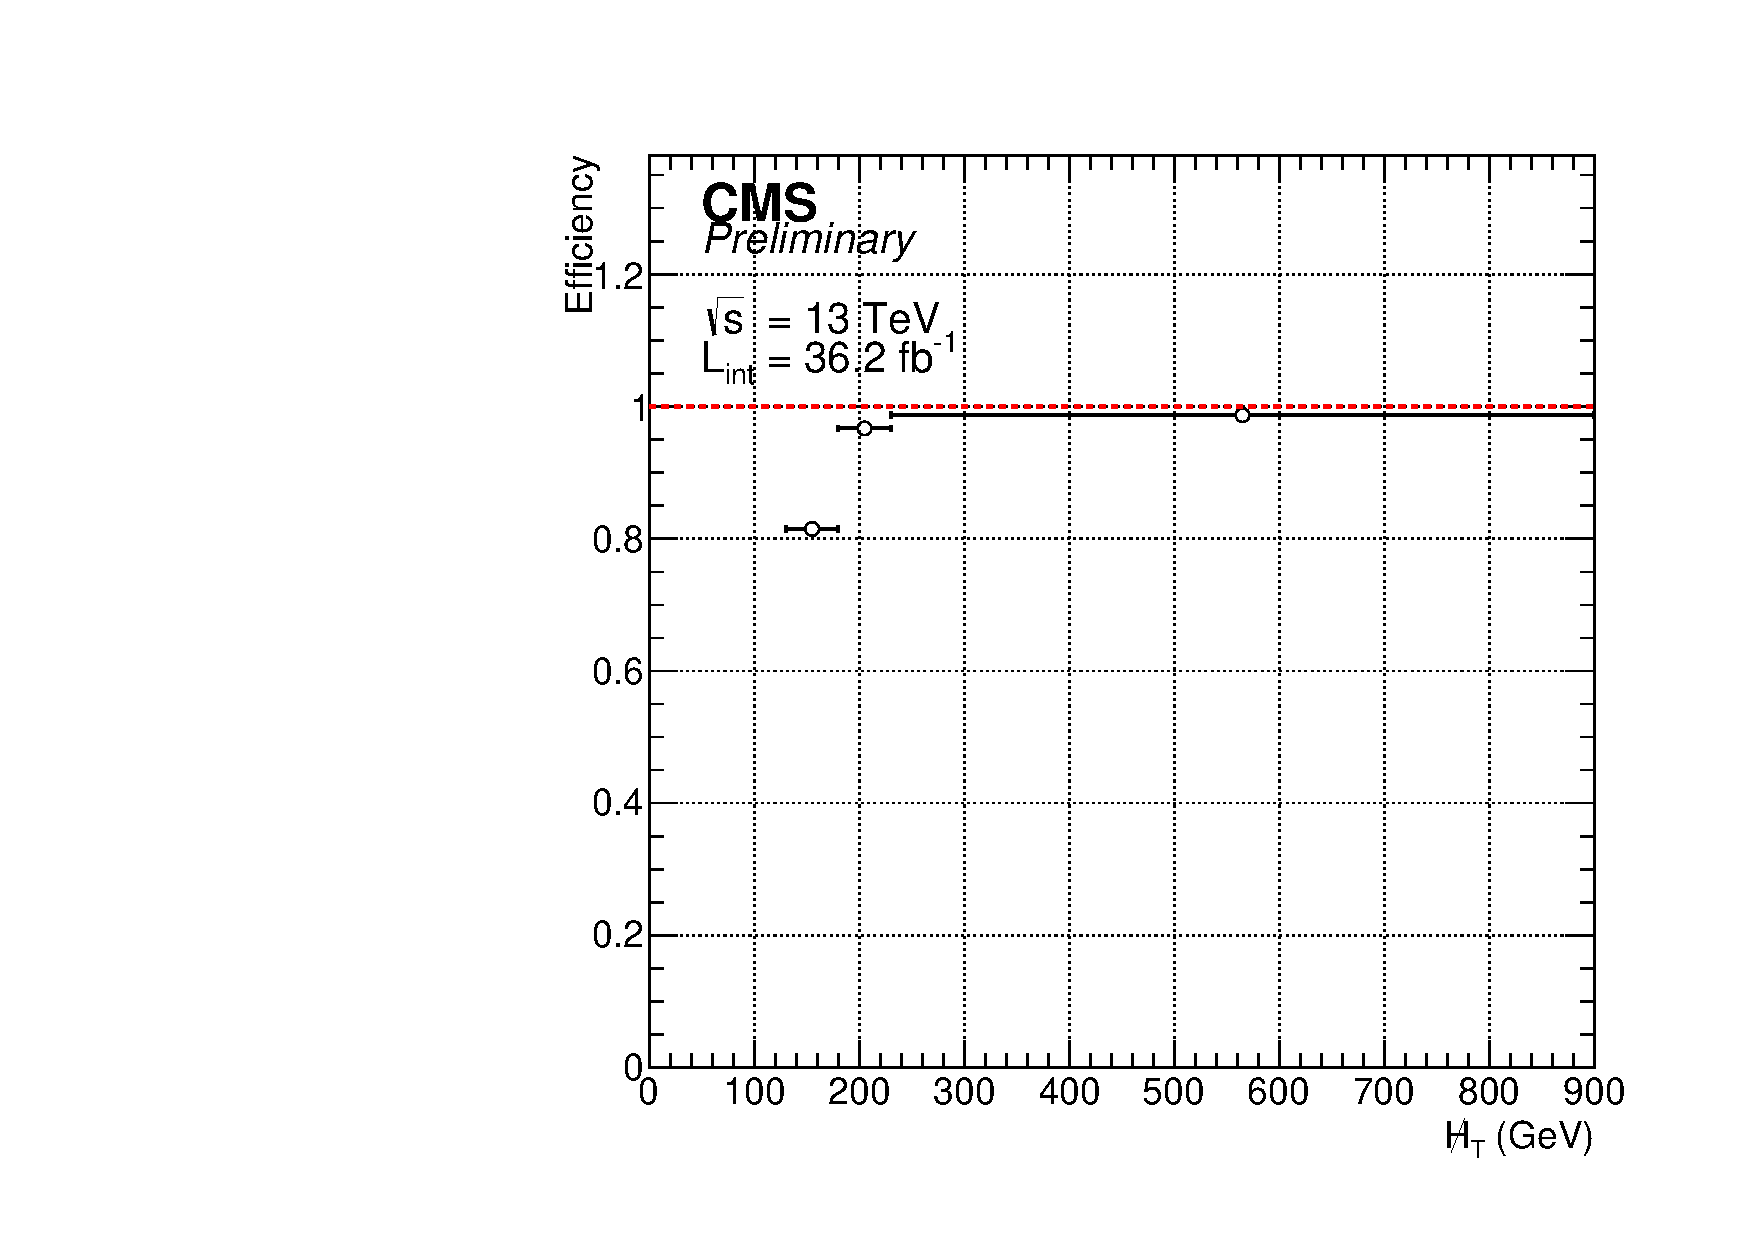
\includegraphics[width=0.28\textwidth]{figures/Trigger/Muon/HLT_AlphaTHT800MonoAll_MoM_all_200to400_mht}} \\
    \subfigure[$400 < \scalht < 600$]{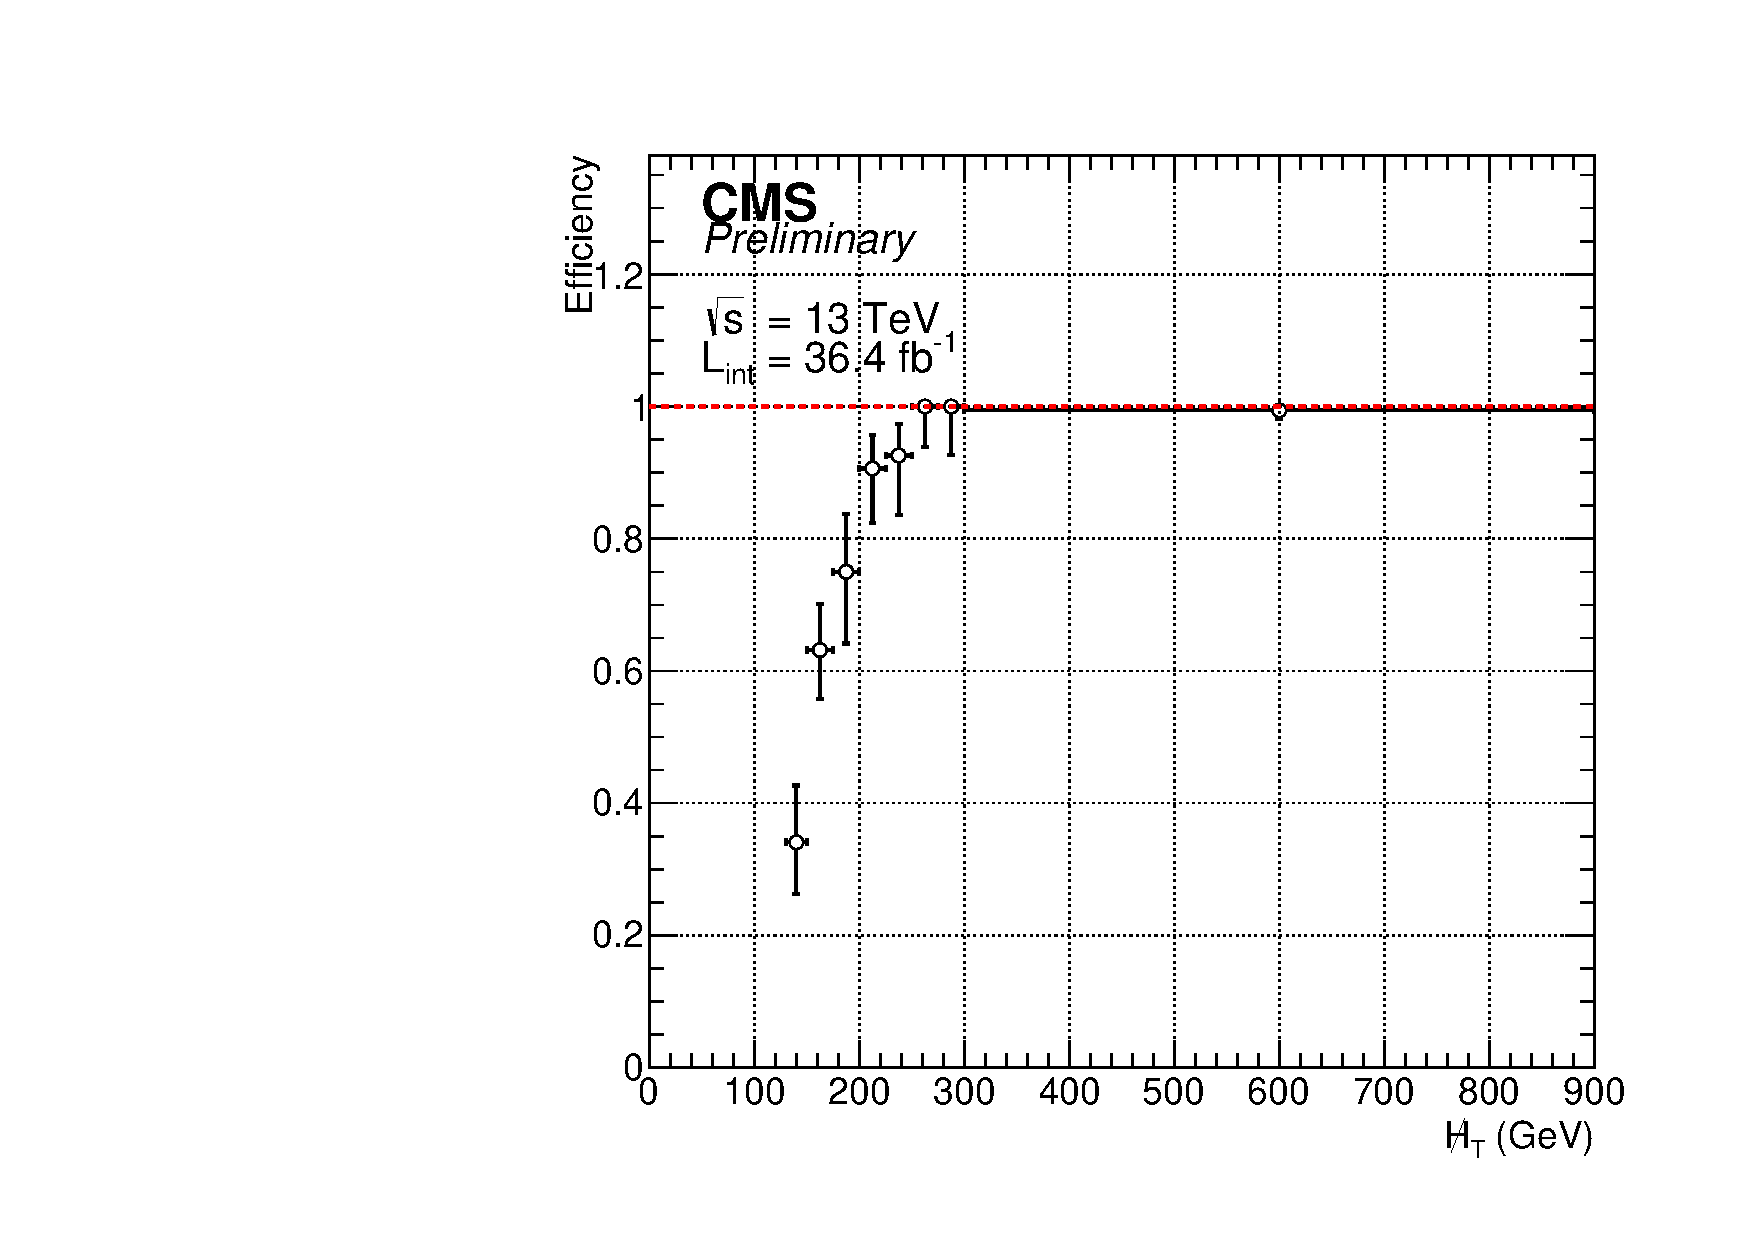
\includegraphics[width=0.28\textwidth]{figures/Trigger/Ele/HLT_AlphaTHT800MonoAll_MoM_all_400to600_mht}} ~
    \subfigure[$400 < \scalht < 600$]{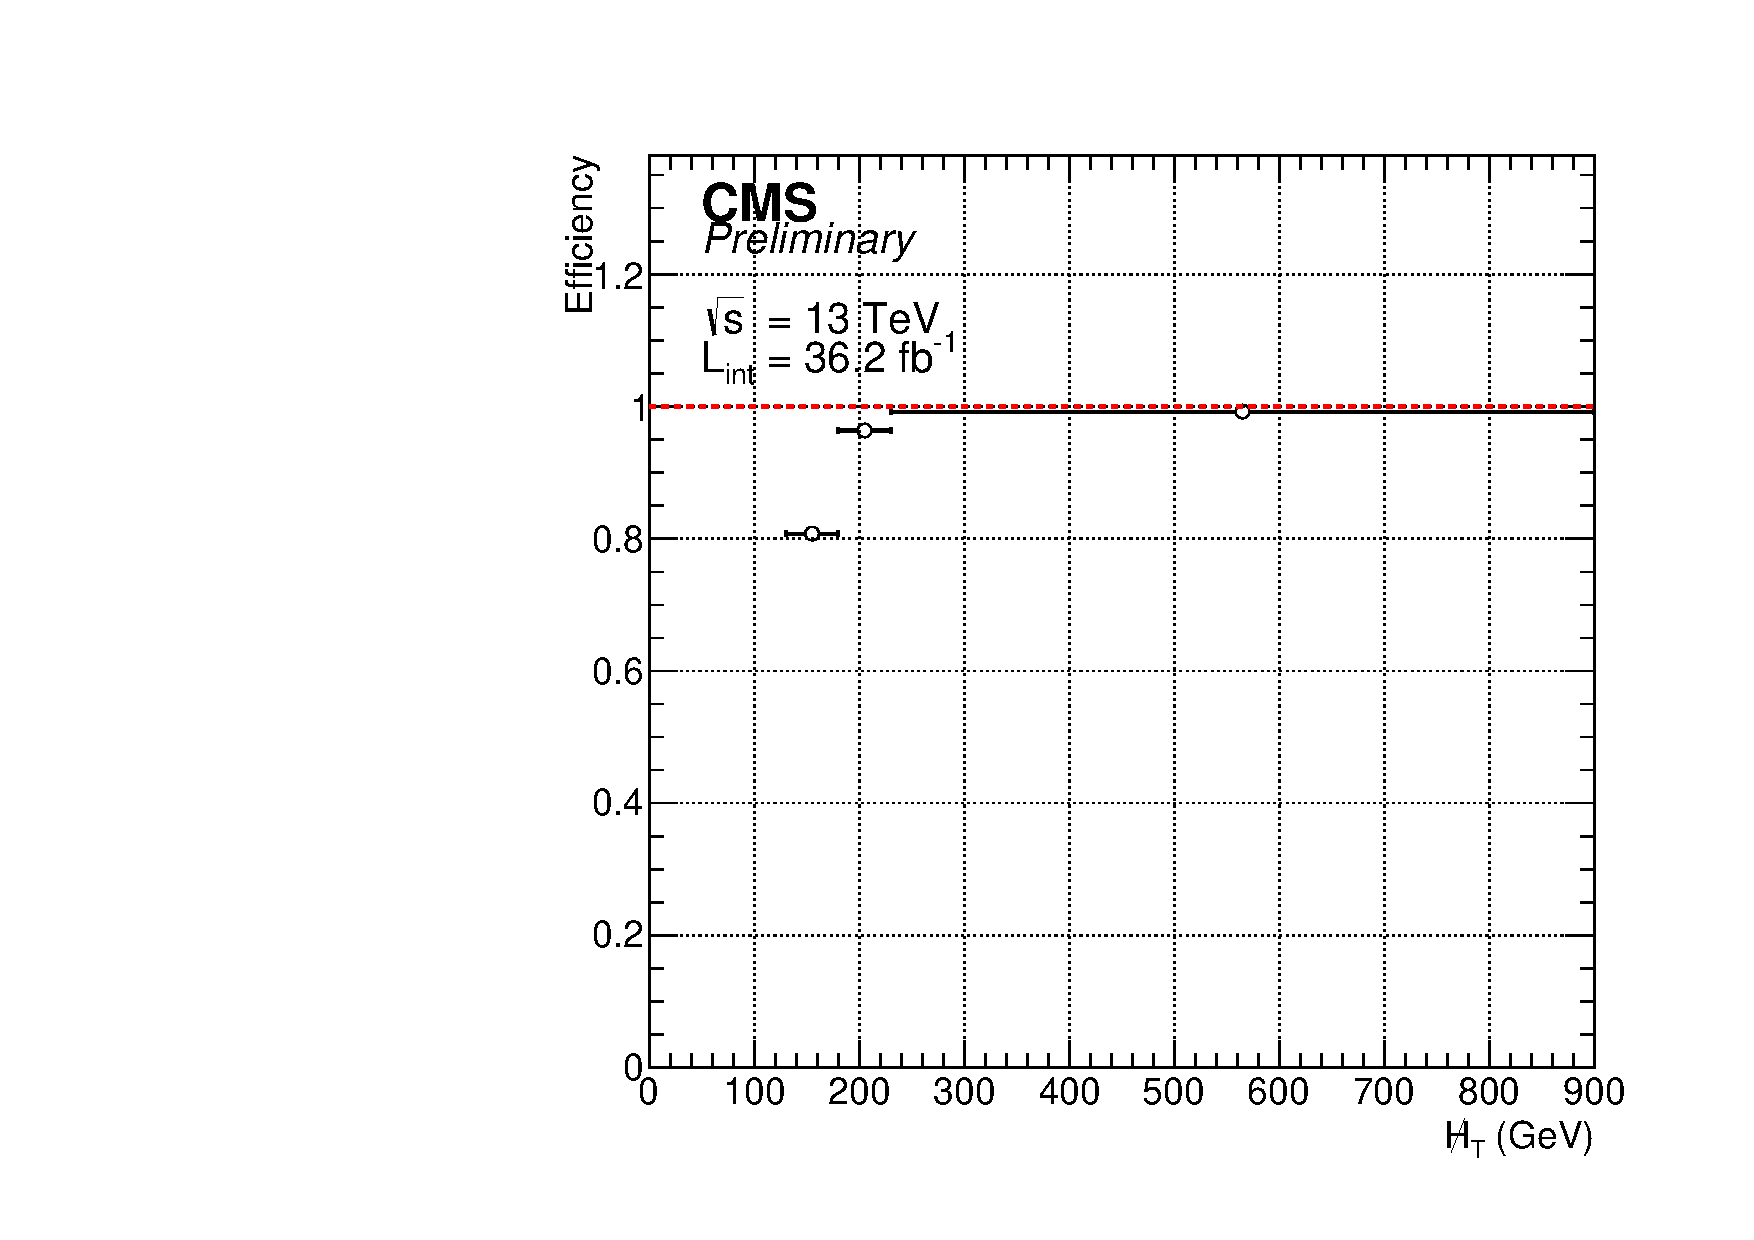
\includegraphics[width=0.28\textwidth]{figures/Trigger/Muon/HLT_AlphaTHT800MonoAll_MoM_all_400to600_mht}} \\
    \subfigure[$600 < \scalht < 900$]{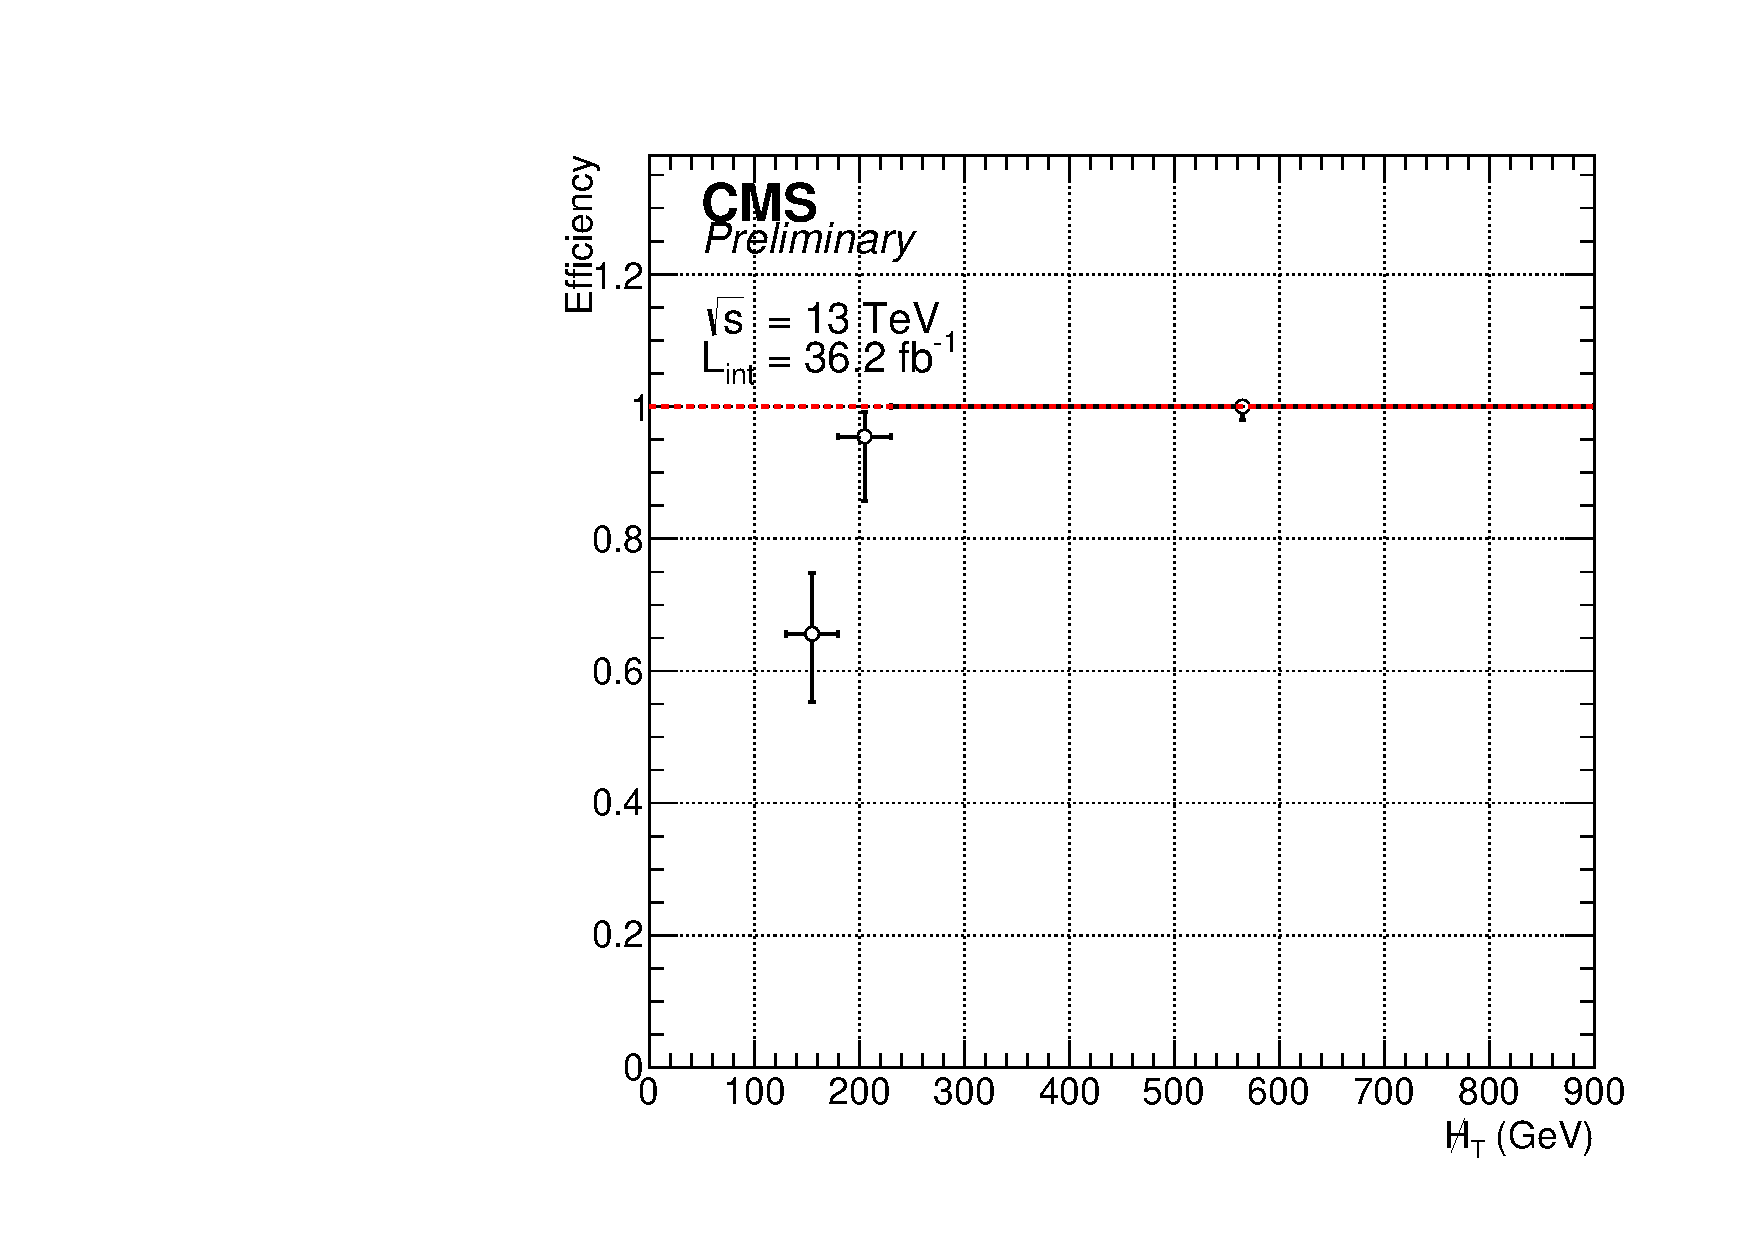
\includegraphics[width=0.28\textwidth]{figures/Trigger/Ele/HLT_AlphaTHT800MonoAll_MoM_all_600to900_mht}} ~
    \subfigure[$600 < \scalht < 900$]{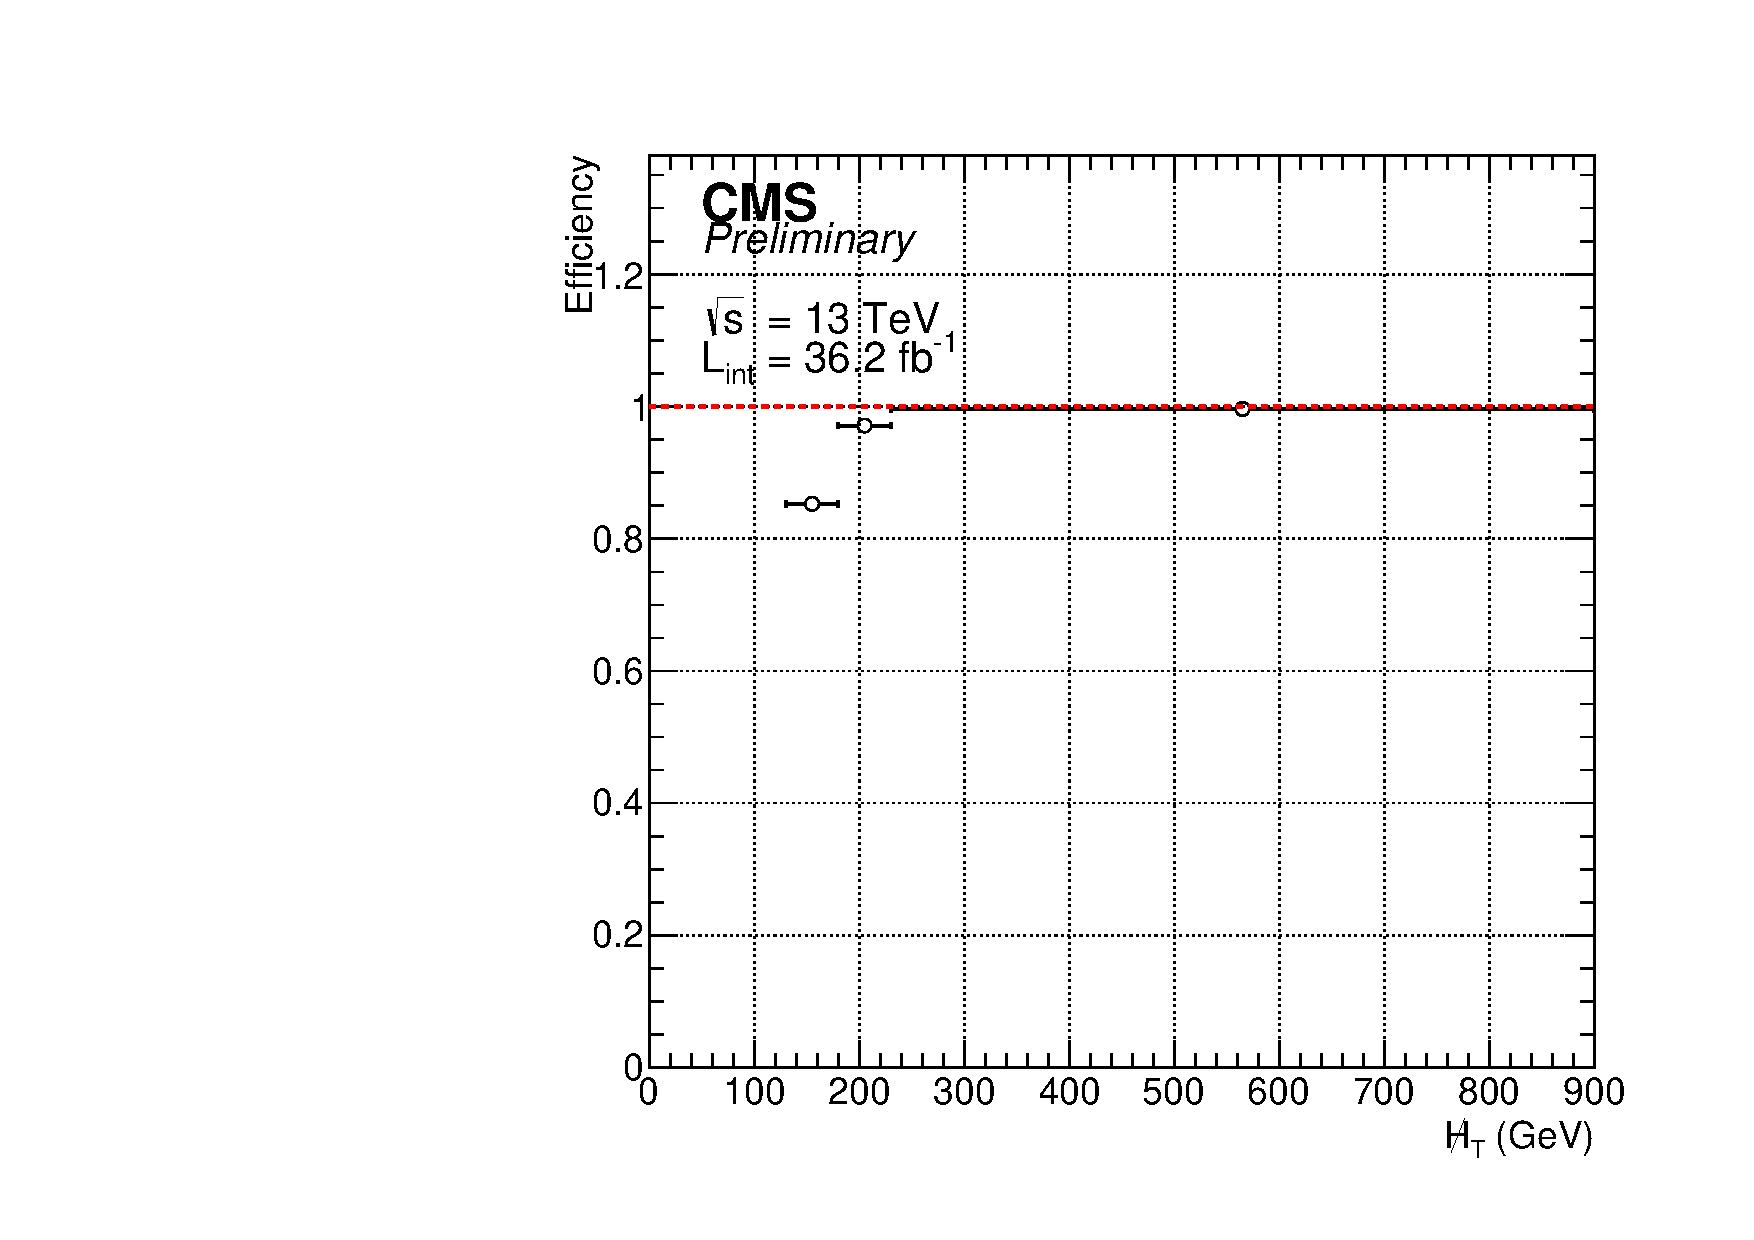
\includegraphics[width=0.28\textwidth]{figures/Trigger/Muon/HLT_AlphaTHT800MonoAll_MoM_all_600to900_mht}} \\
    \subfigure[$\scalht > 900$]      {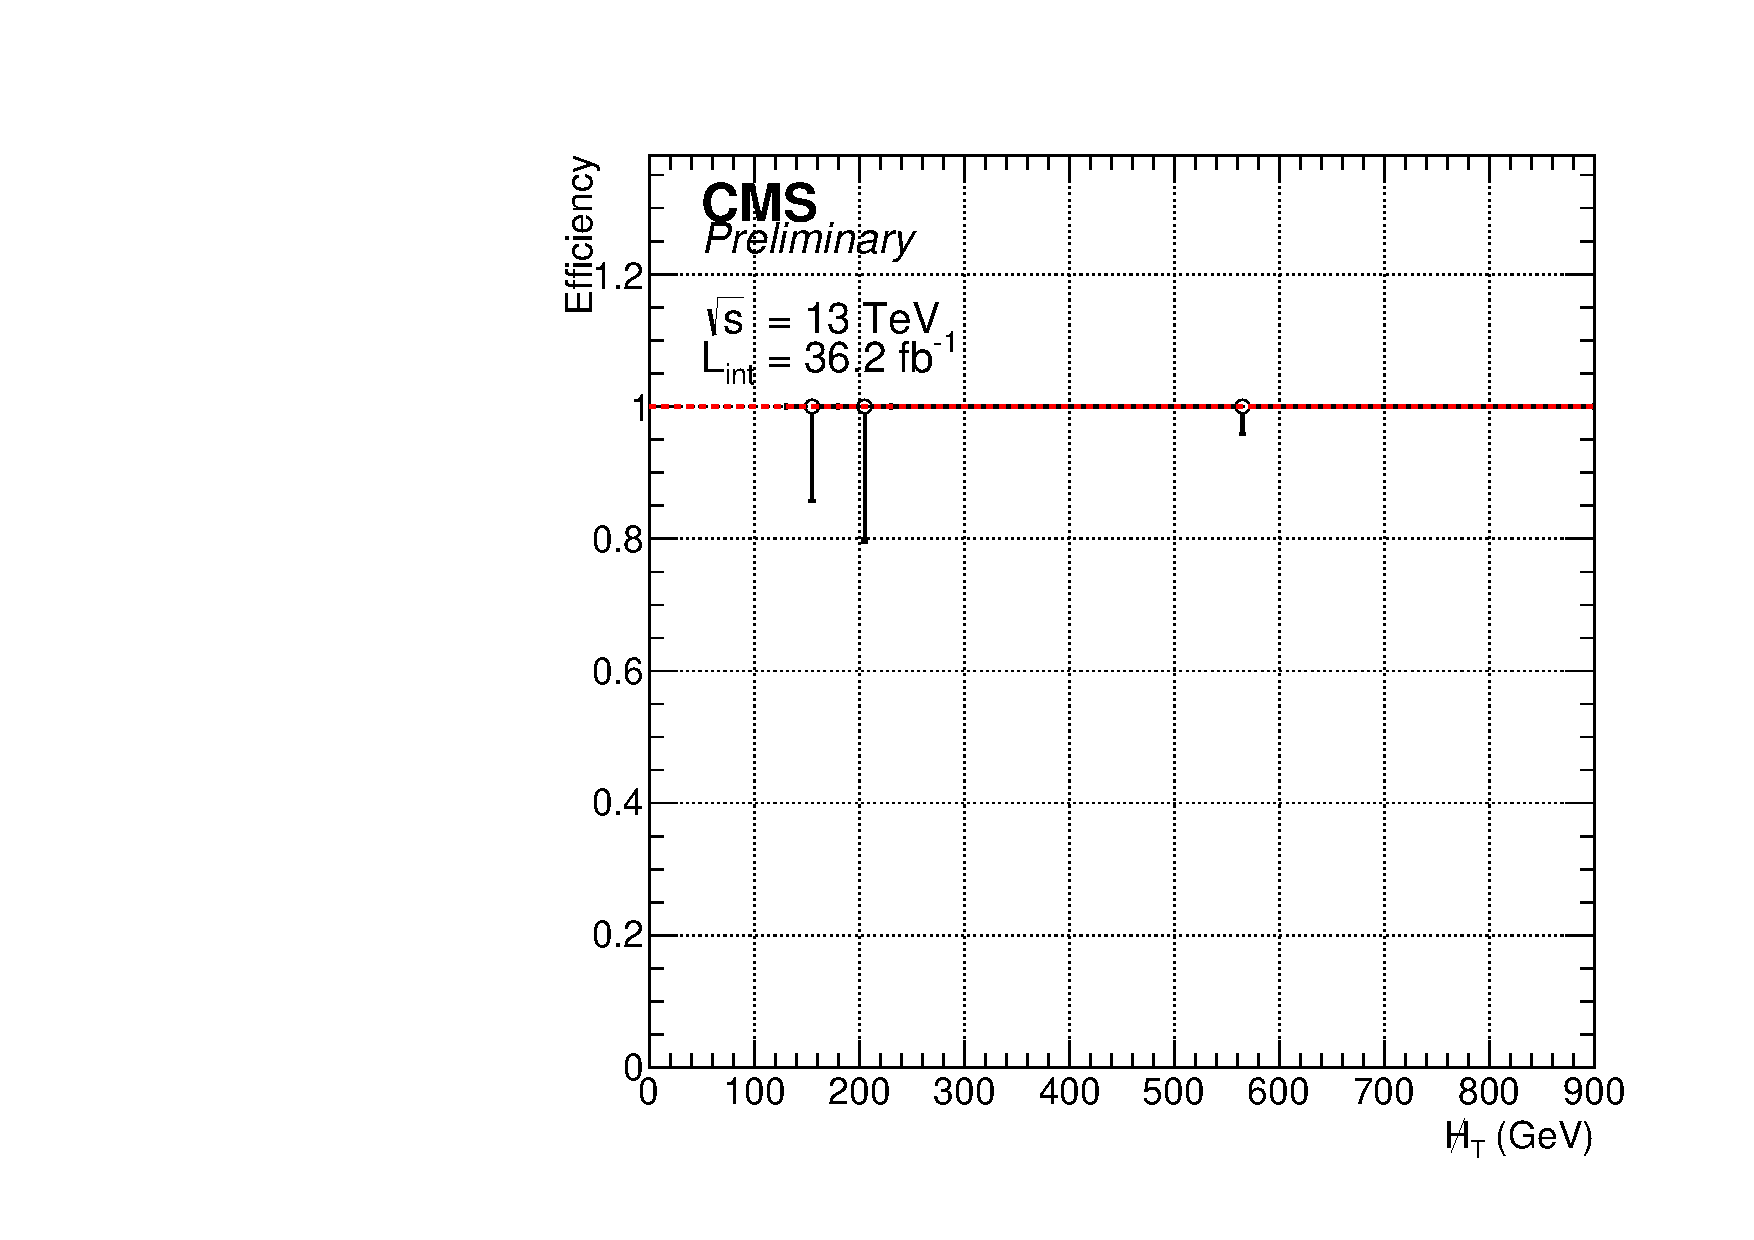
\includegraphics[width=0.28\textwidth]{figures/Trigger/Ele/HLT_AlphaTHT800MonoAll_MoM_all_900to999999_mht}} ~
    \subfigure[$\scalht > 900$]      {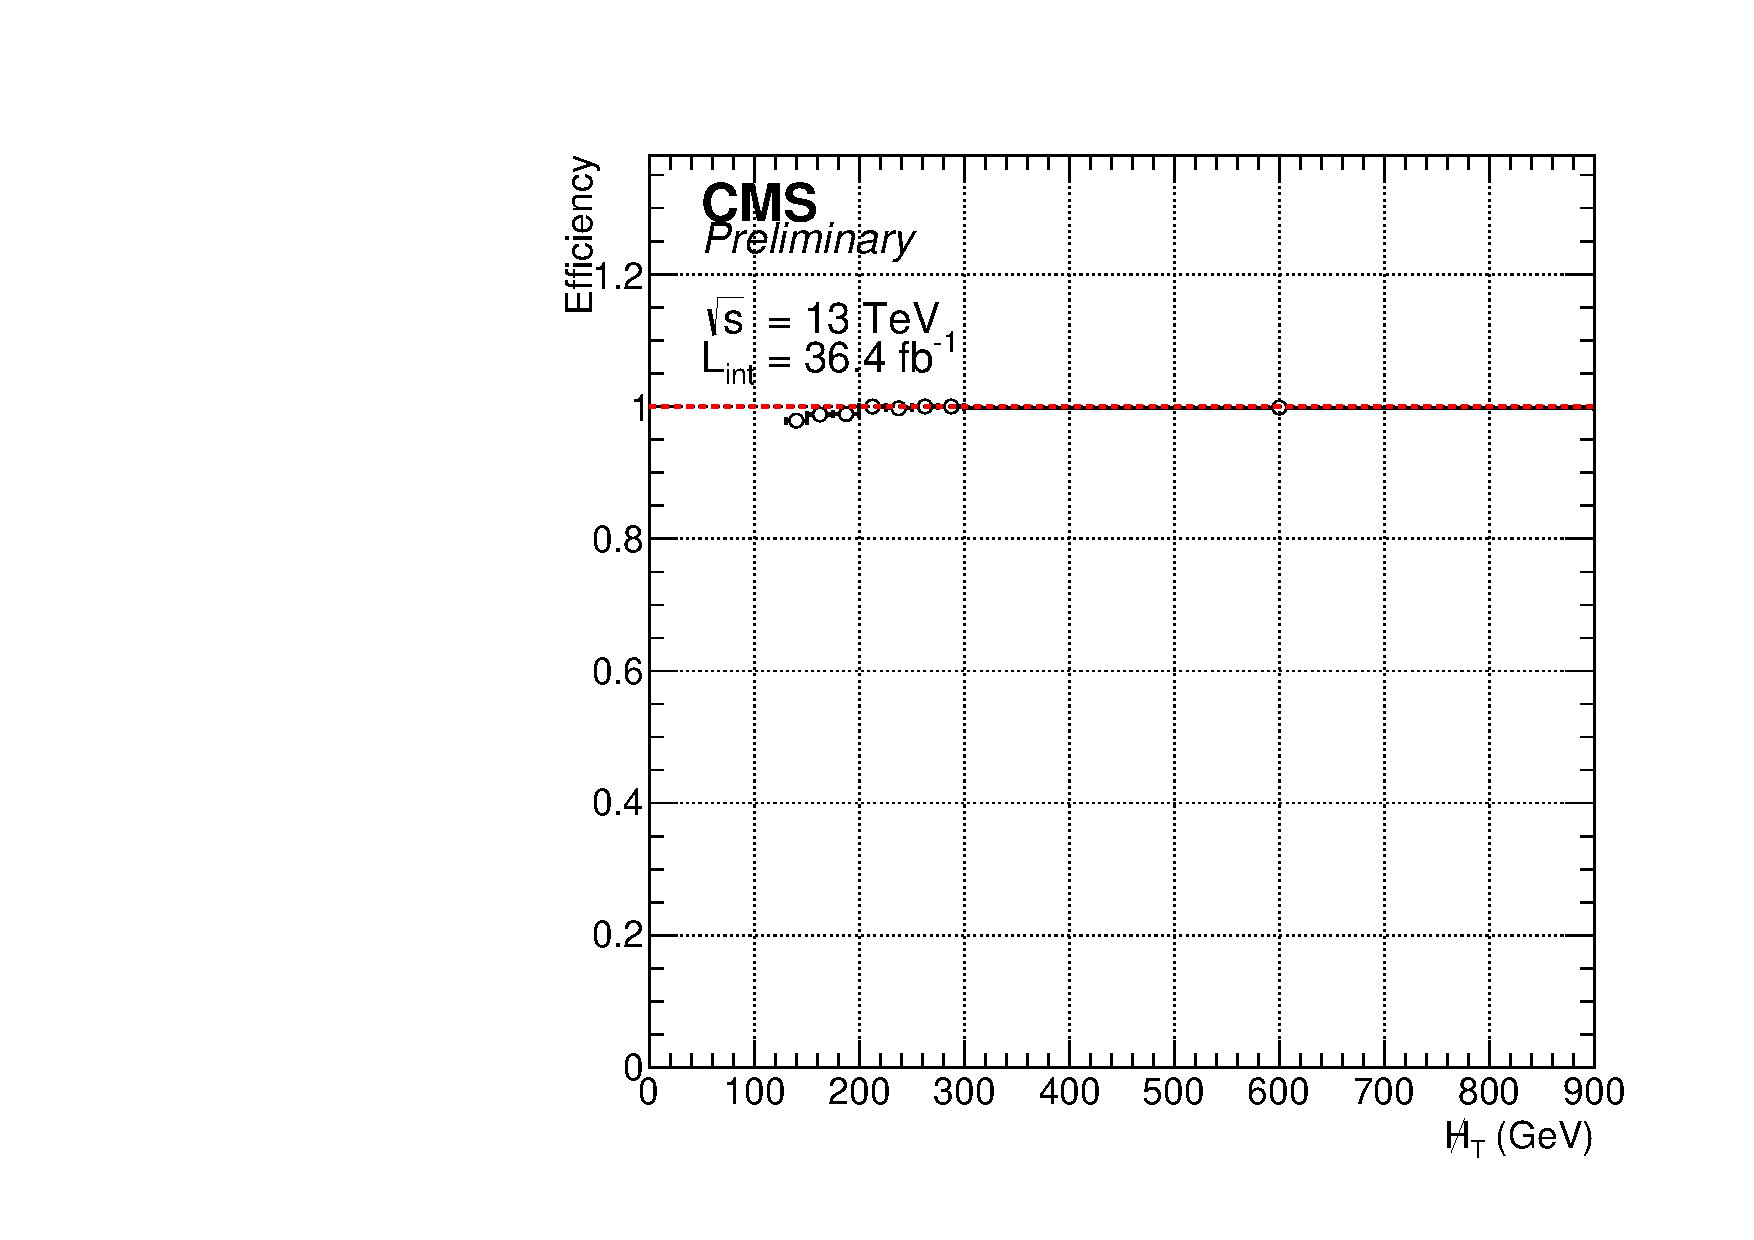
\includegraphics[width=0.28\textwidth]{figures/Trigger/Muon/HLT_AlphaTHT800MonoAll_MoM_all_900to999999_mht}} 
    \caption{Signal trigger efficiency in the \mht dimension
      determined from data using a ``reference'' event sample
      containing (left) an electron or (right) a muon.}
    \label{fig:alphat_turnons}
  \end{center}
\end{figure}

\begin{figure}[h!]
  \begin{center}
    \subfigure{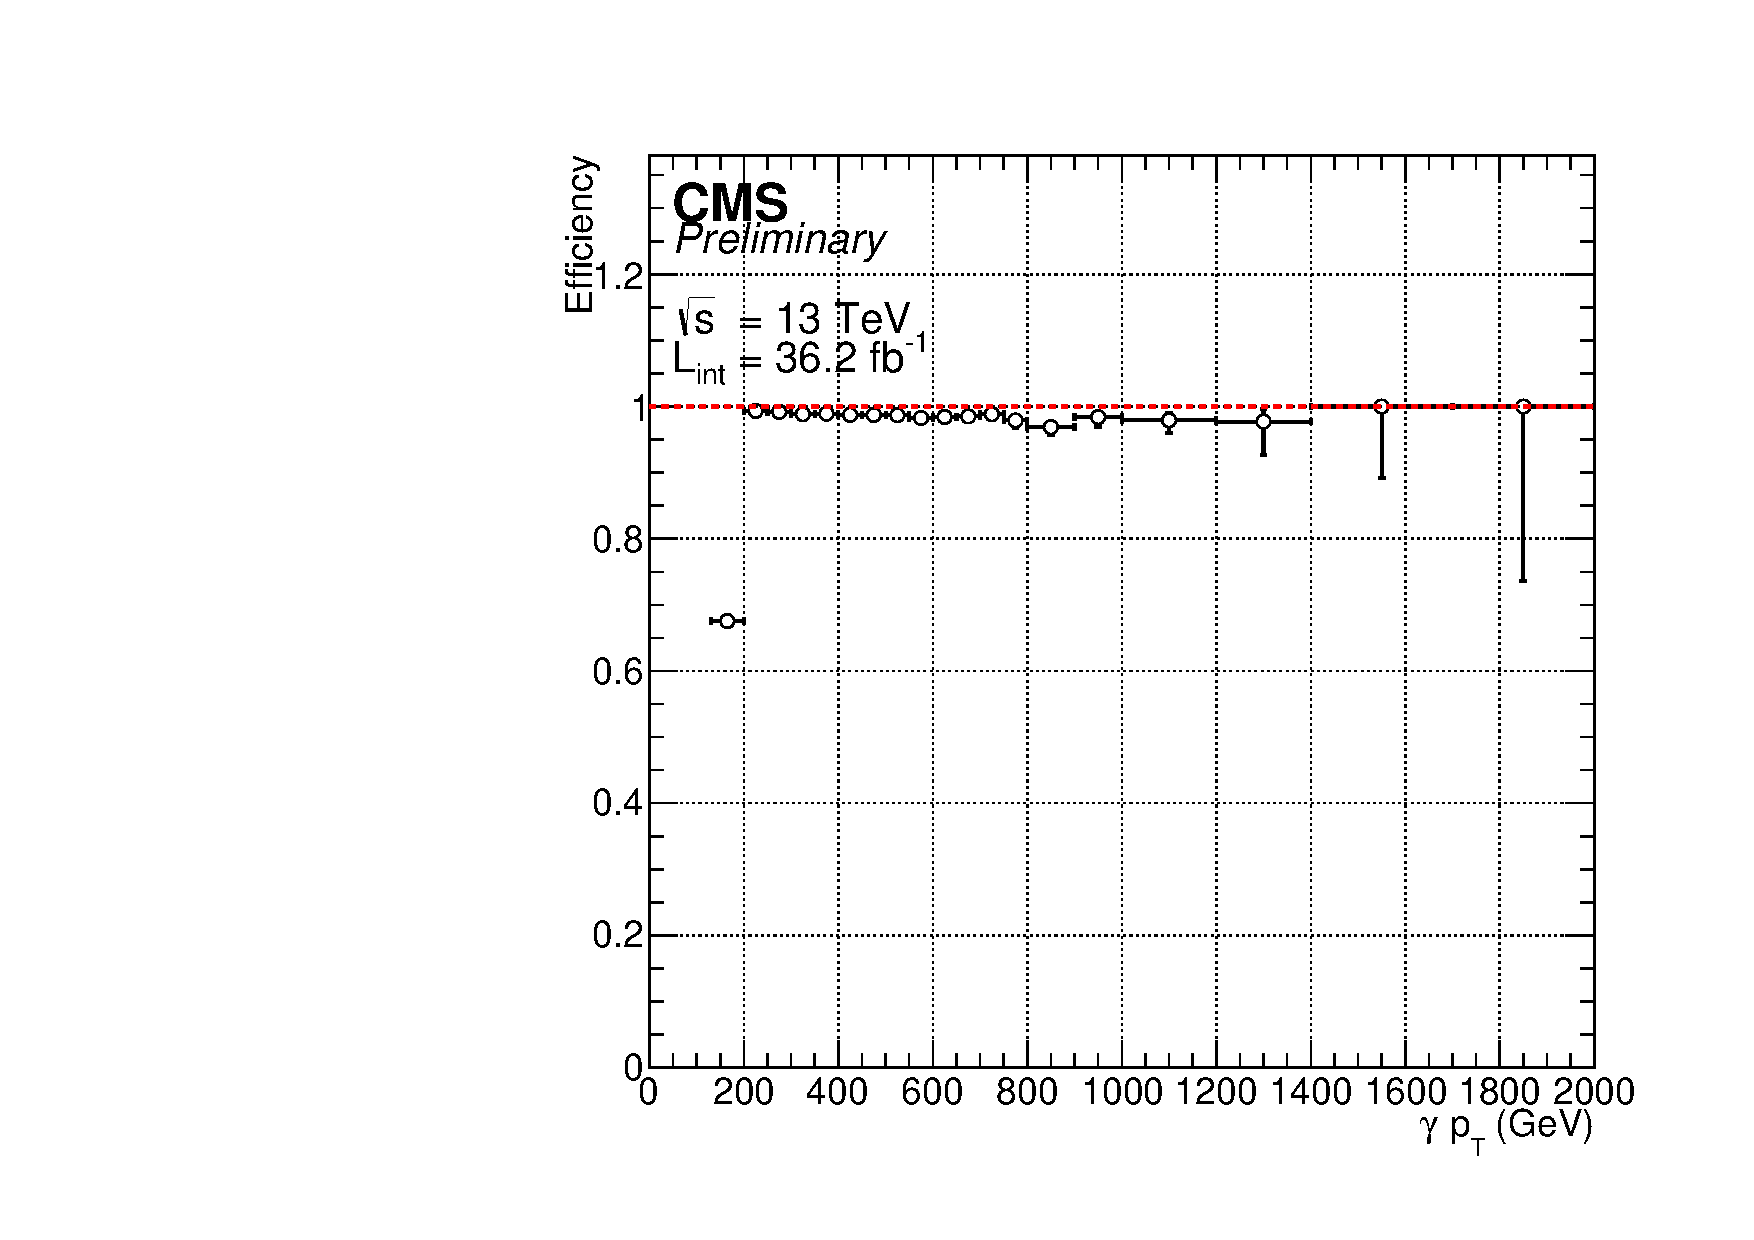
\includegraphics[width=0.45\textwidth]{figures/Trigger/Photon/HLT_Photon175_MoM_all_all_gammapt}} ~
    \subfigure{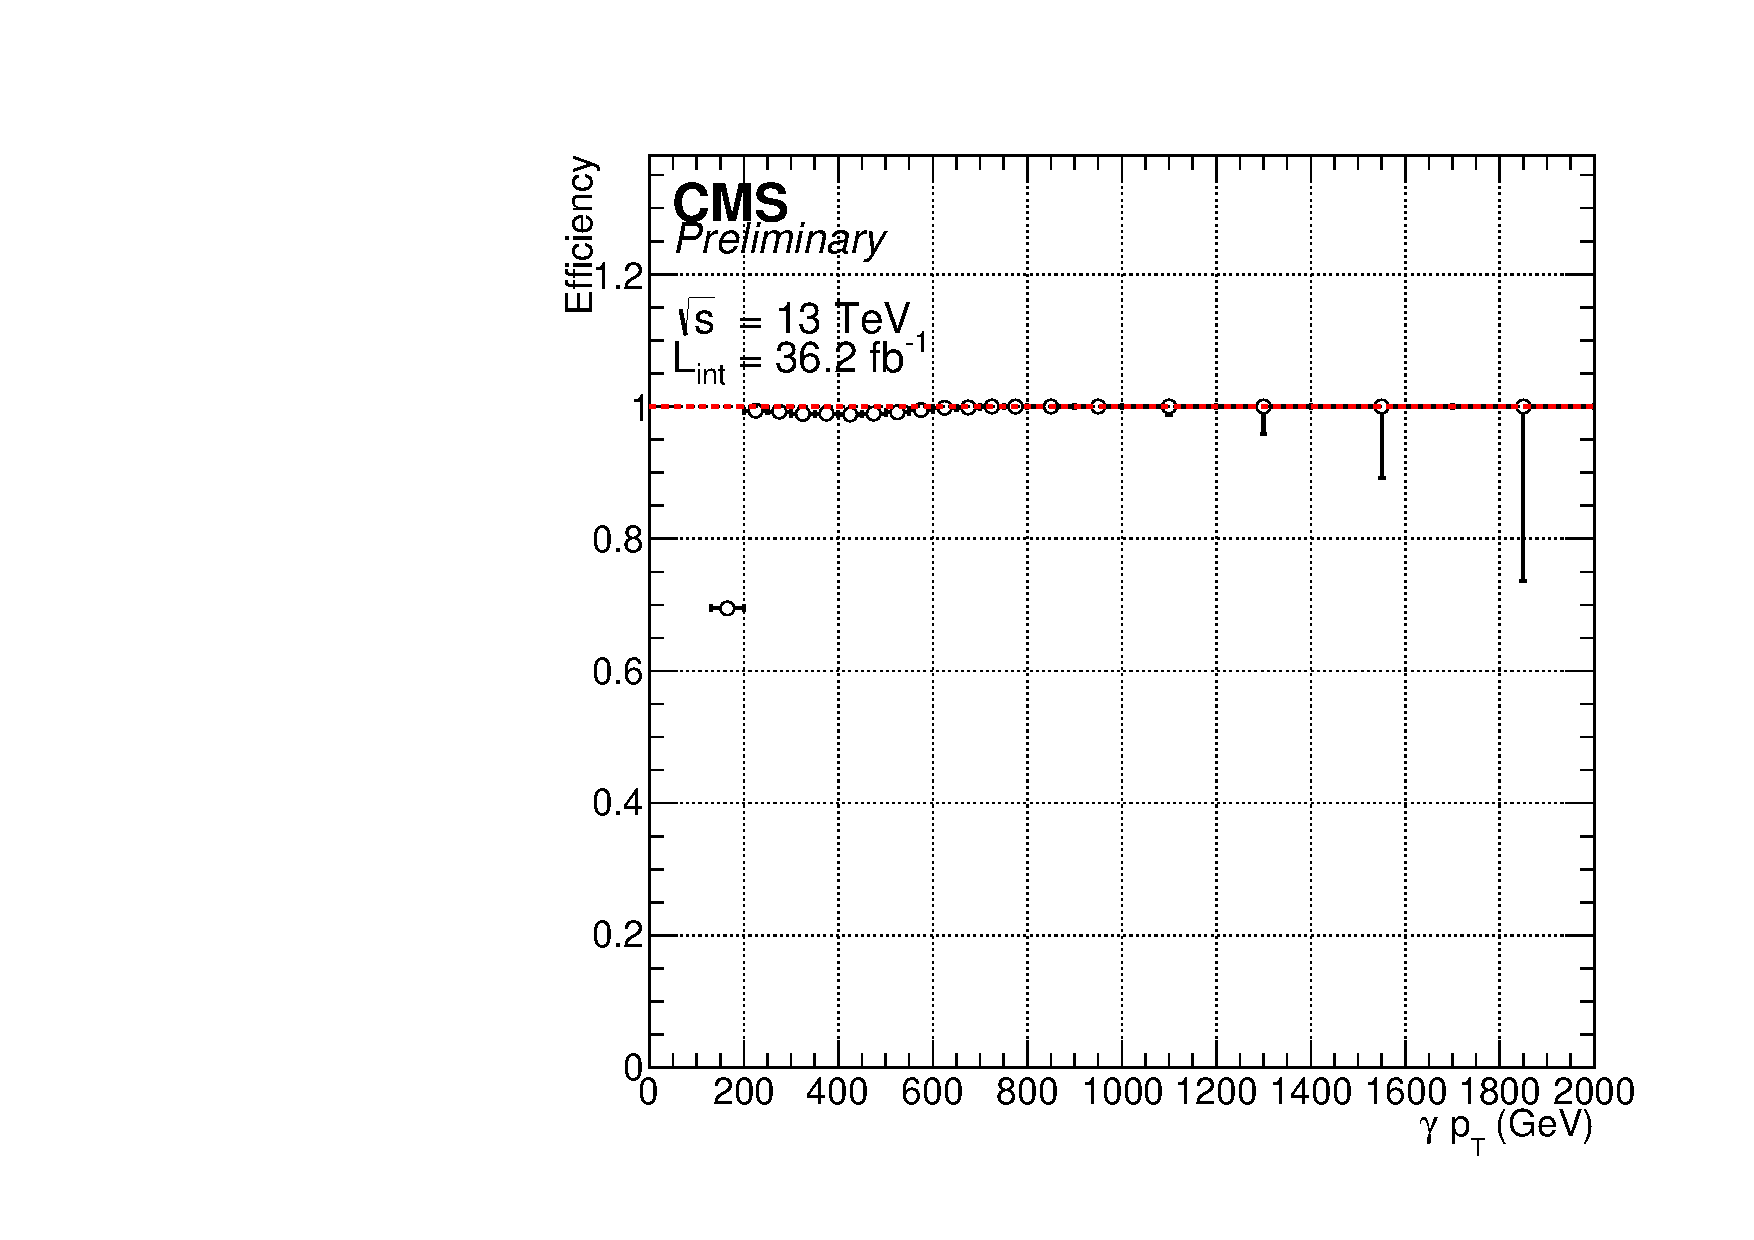
\includegraphics[width=0.45\textwidth]{figures/Trigger/Photon/HLT_PhotonECALHT800_MoM_all_all_gammapt}} \\
    \subfigure{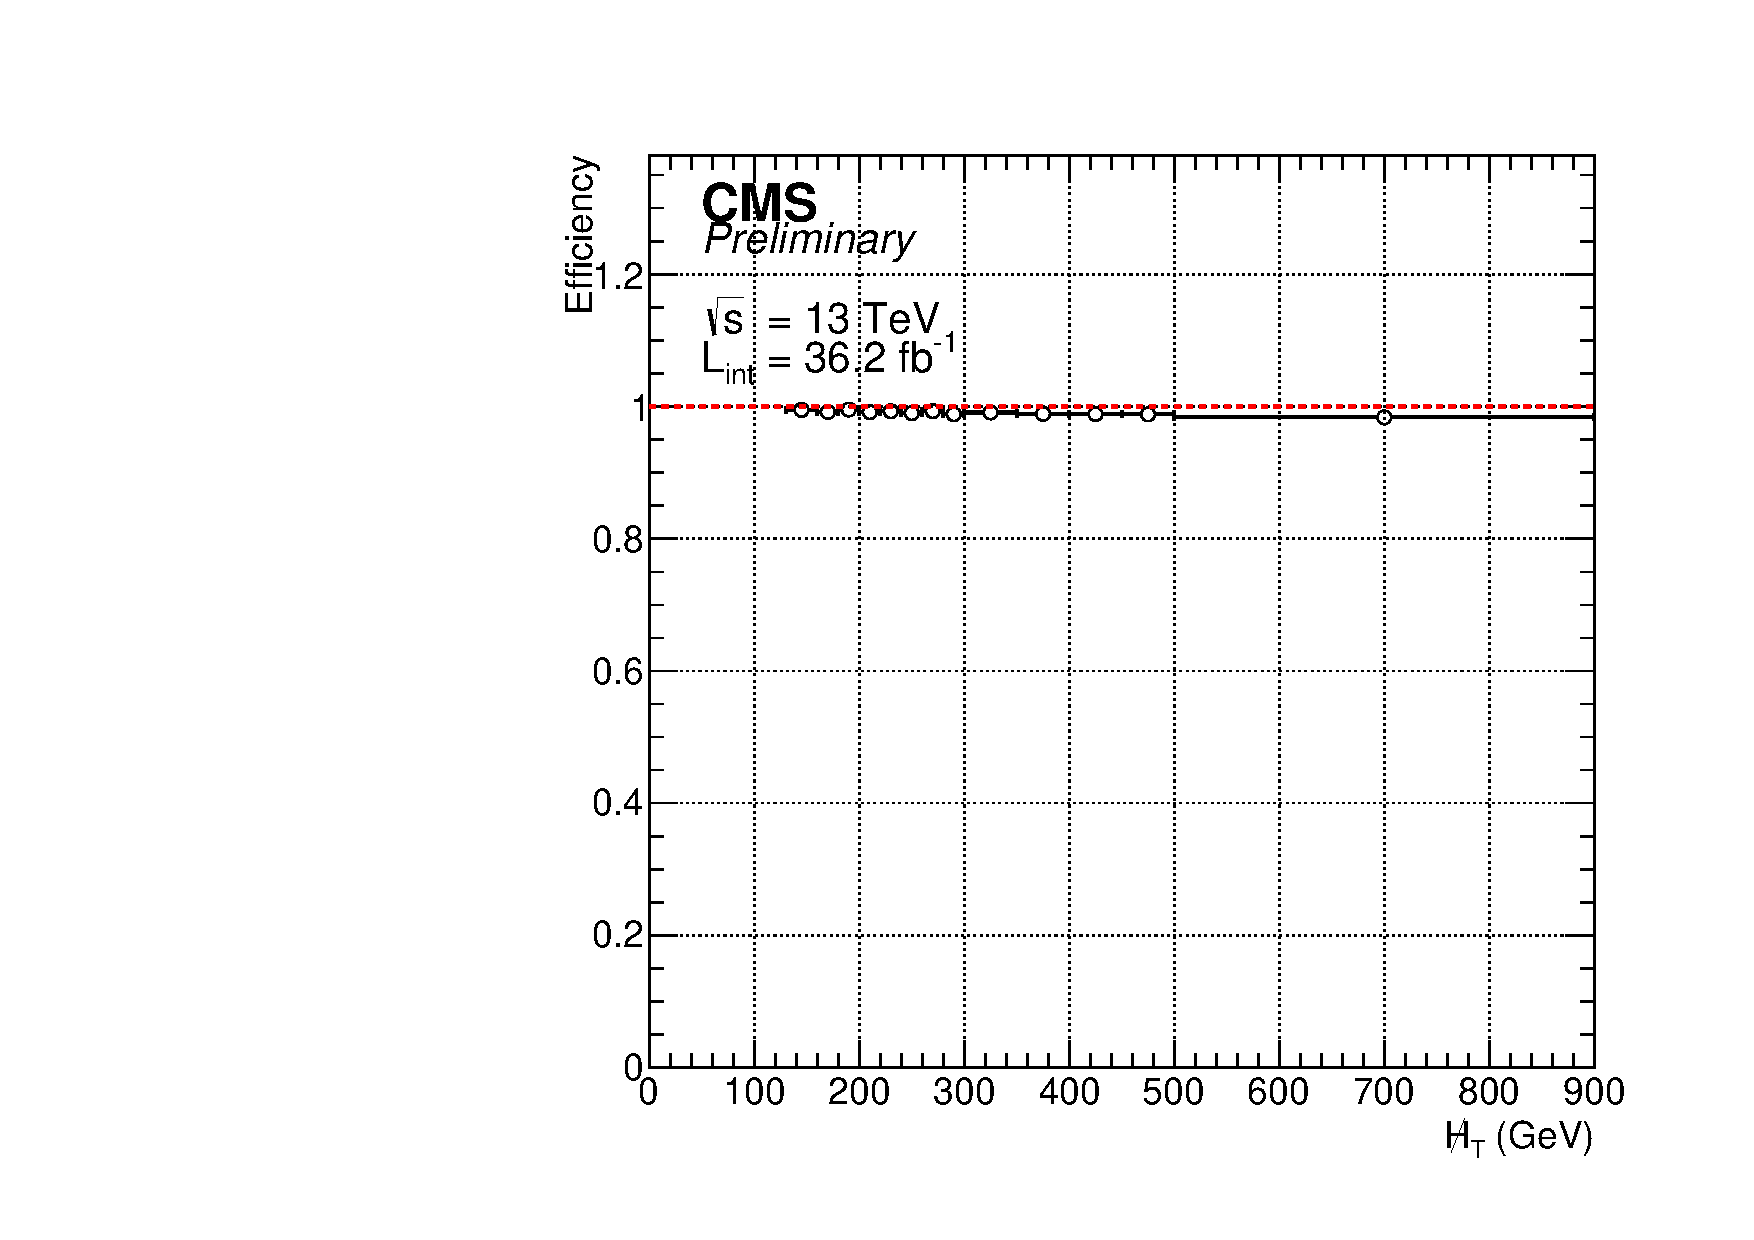
\includegraphics[width=0.45\textwidth]{figures/Trigger/Photon/HLT_Photon175_MoM_all_all_mht}} ~
    \subfigure{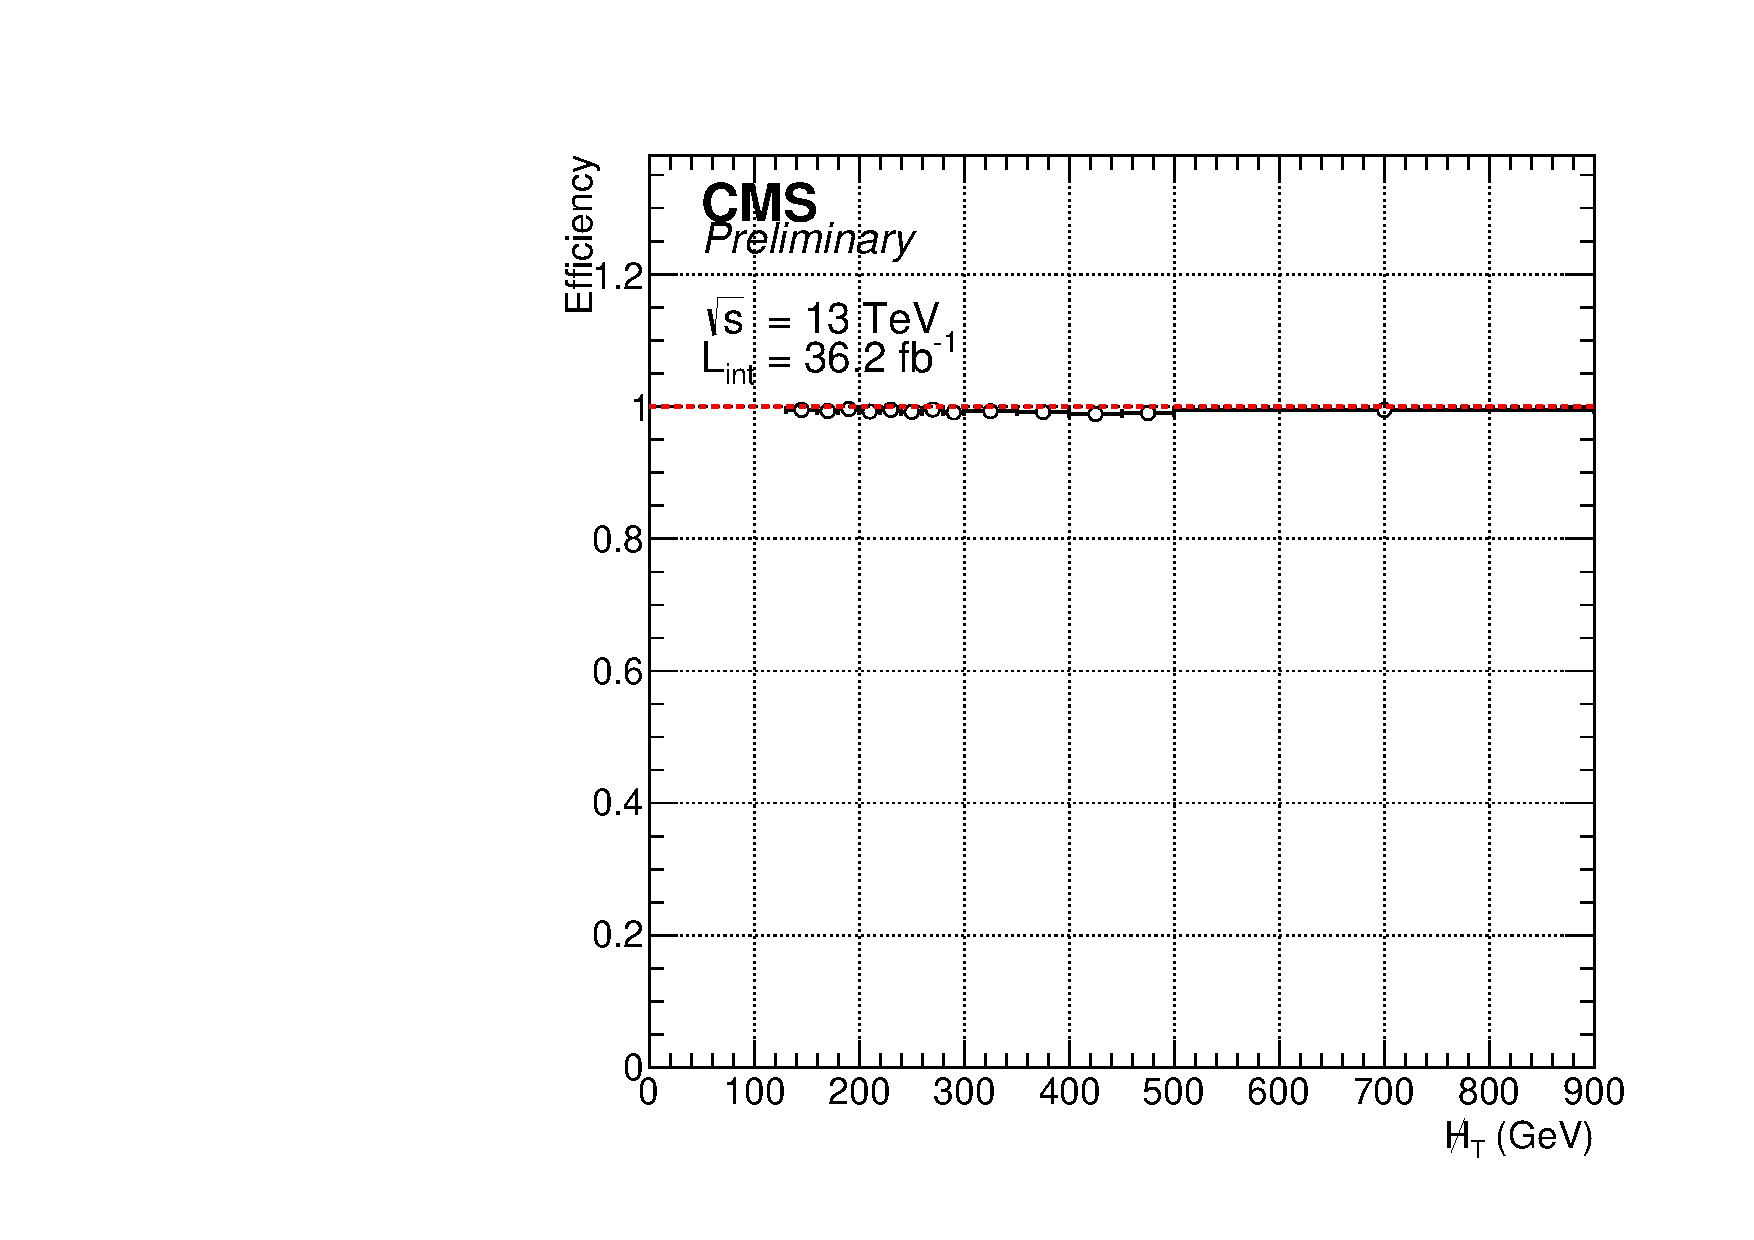
\includegraphics[width=0.45\textwidth]{figures/Trigger/Photon/HLT_PhotonECALHT800_MoM_all_mht}} \\
    \caption{Trigger efficiency as a function of (top) photon \Pt or
      (bottom) \HTmiss for (left) \texttt{Photon175} and (right)
      \texttt{Photon175 or ECALHT800}, measured with events in the
      \texttt{JetHT} primary data set that satisfy the \gj control
      region event selection criteria. }
    \label{fig:photon_turnons_photonPt}
  \end{center}
\end{figure}

%\begin{figure}[h!]
%  \begin{center}
%    \subfigure{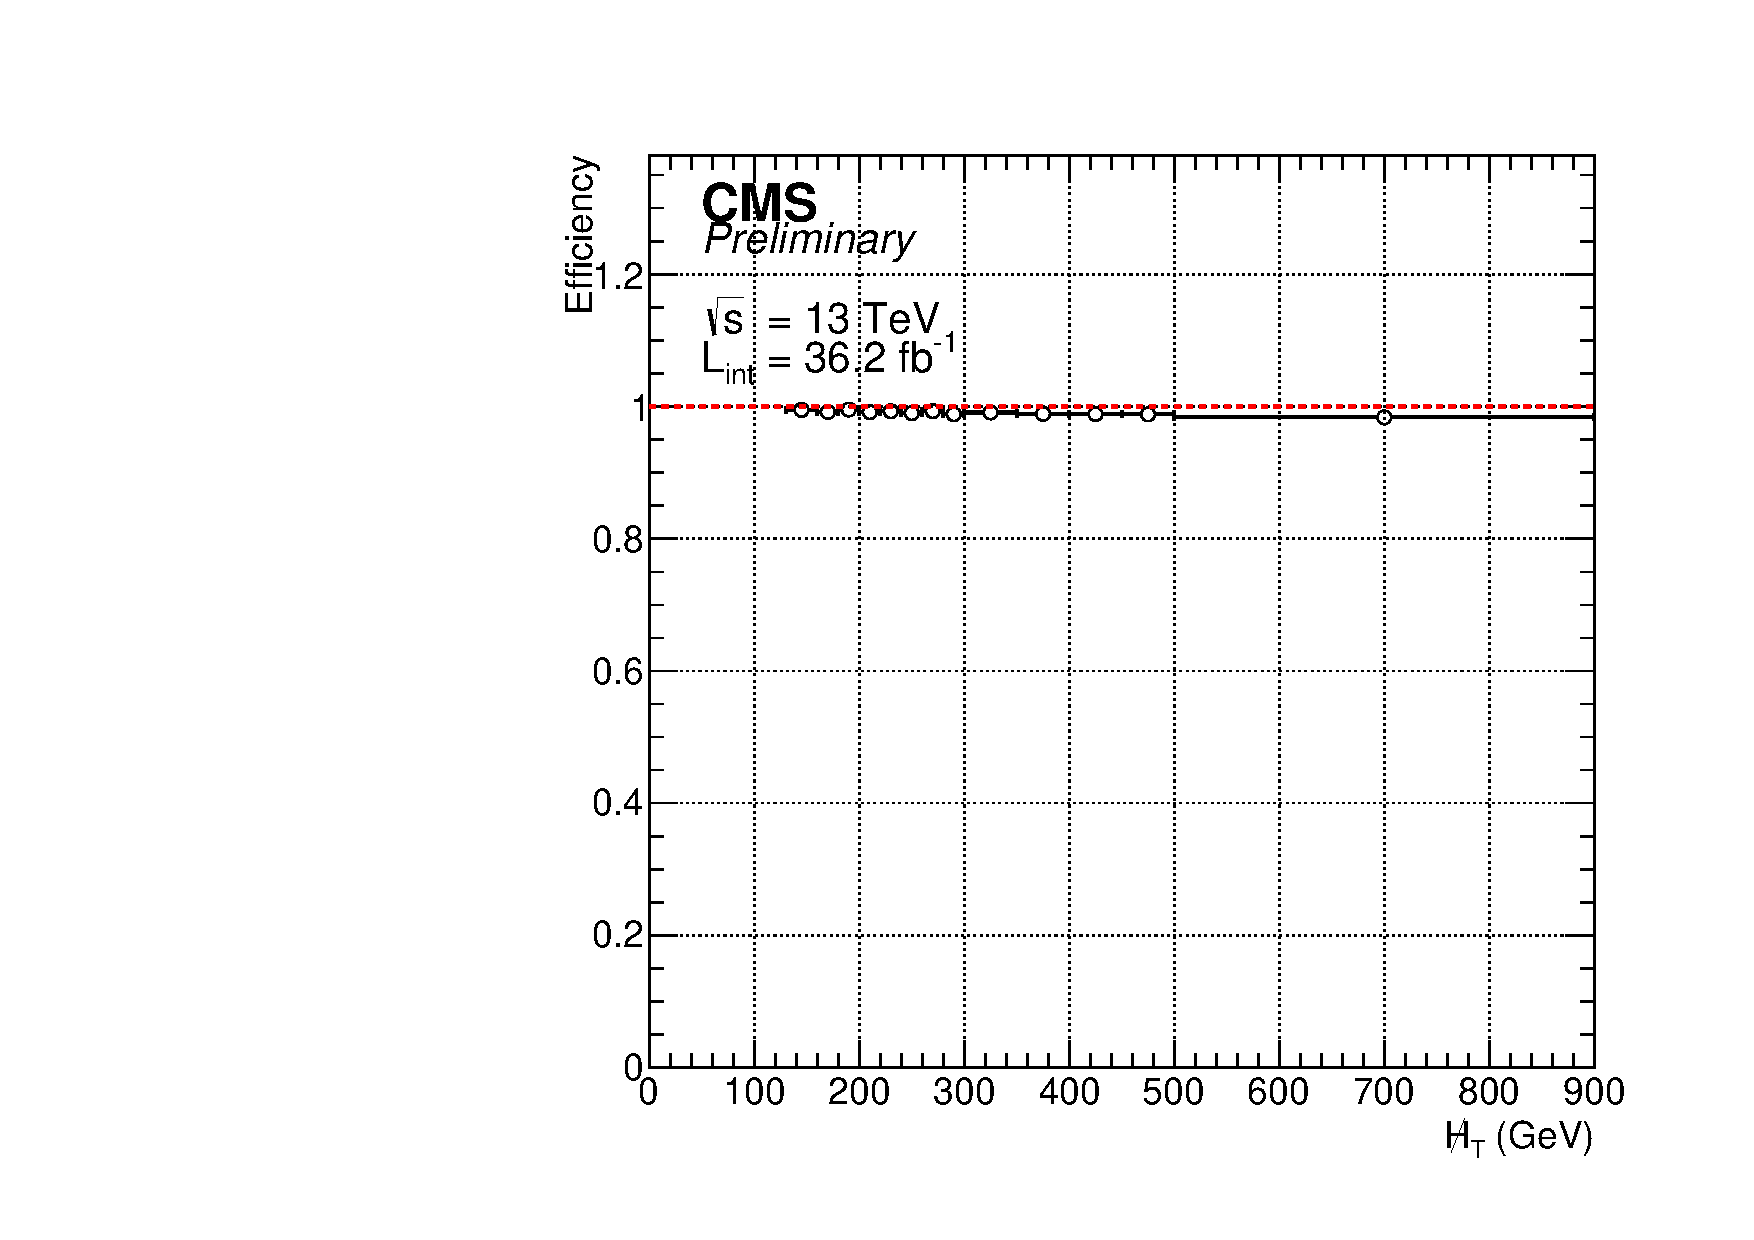
\includegraphics[width=0.4\textwidth]{figures/Trigger/Photon/HLT_Photon175_MoM_all_all_mht}} ~~\
%    \subfigure{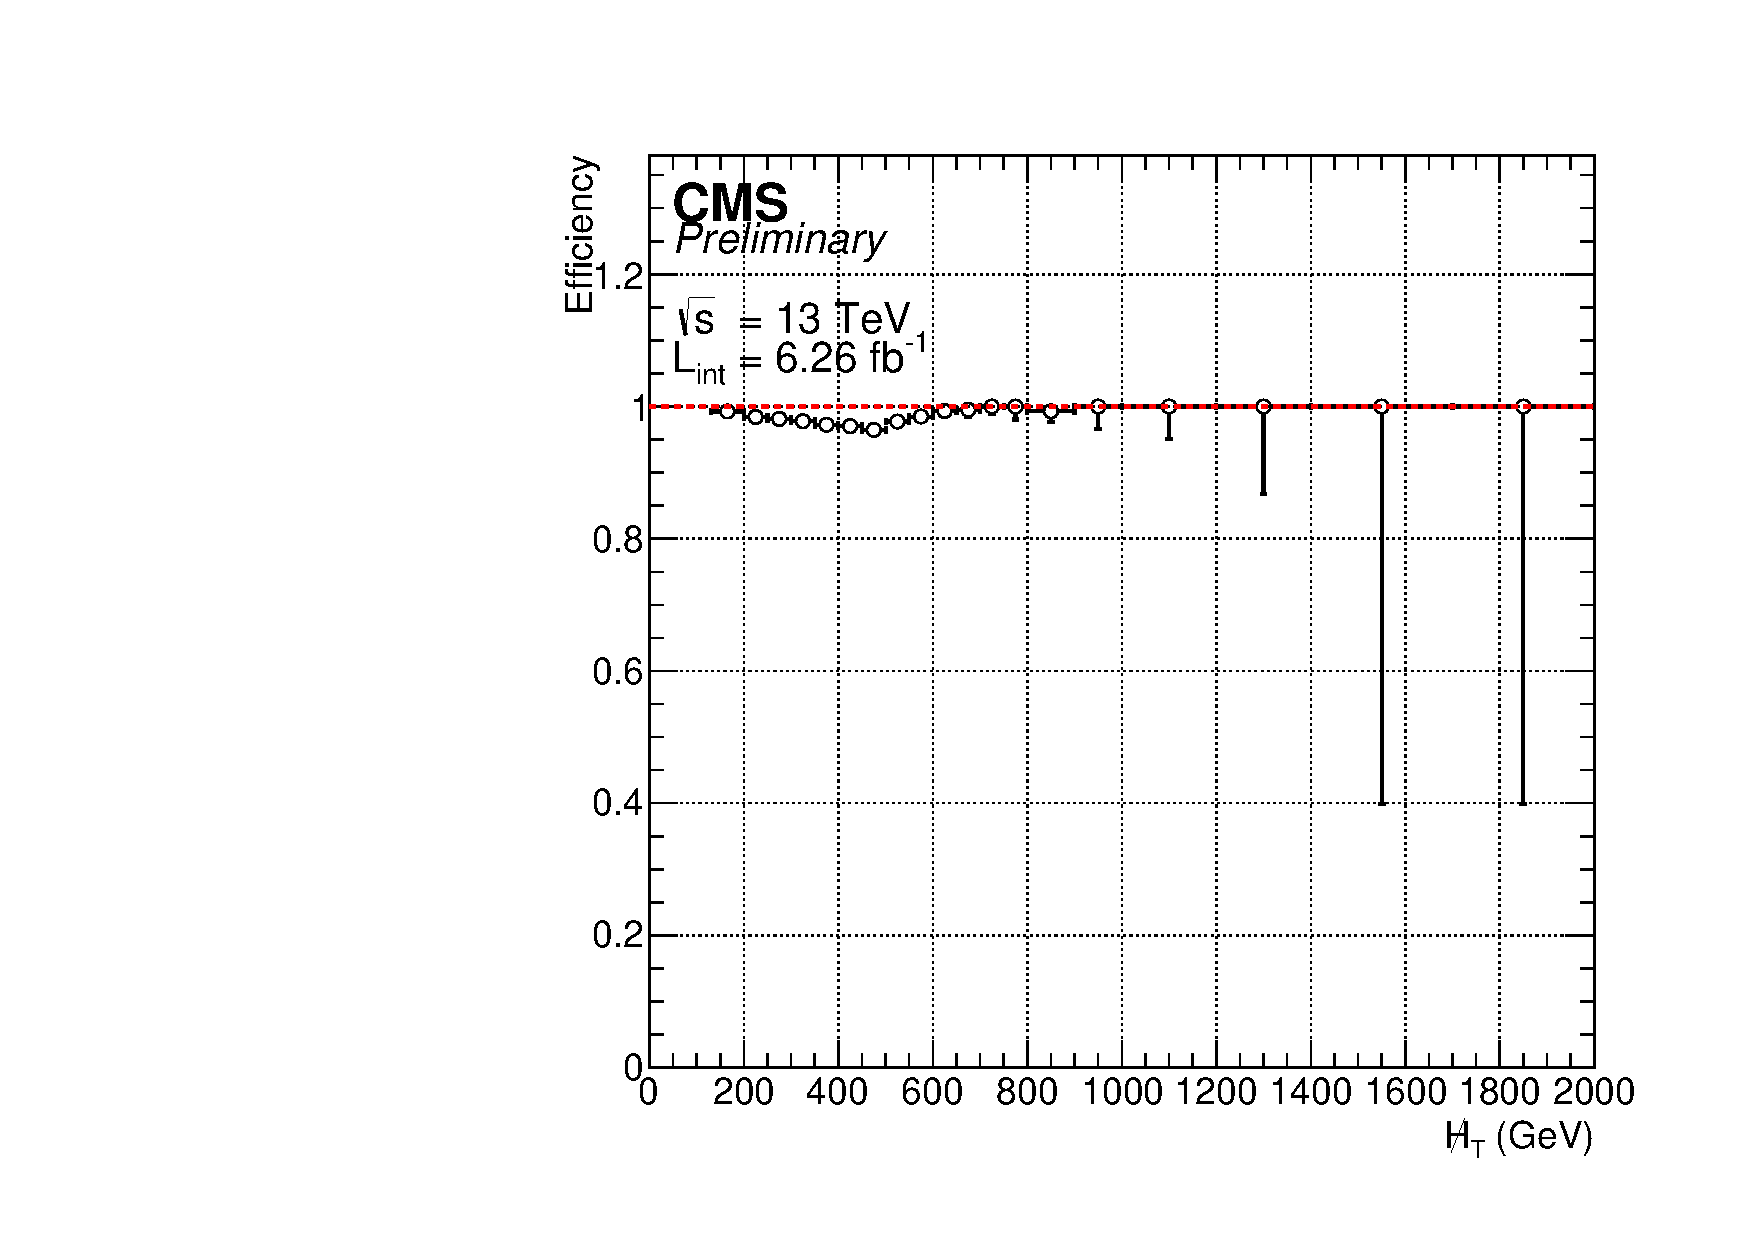
\includegraphics[width=0.4\textwidth]{figures/Trigger/Photon/HLT_PhotonECALHT800_MoM_all_all_mht}} \\
%    \subfigure{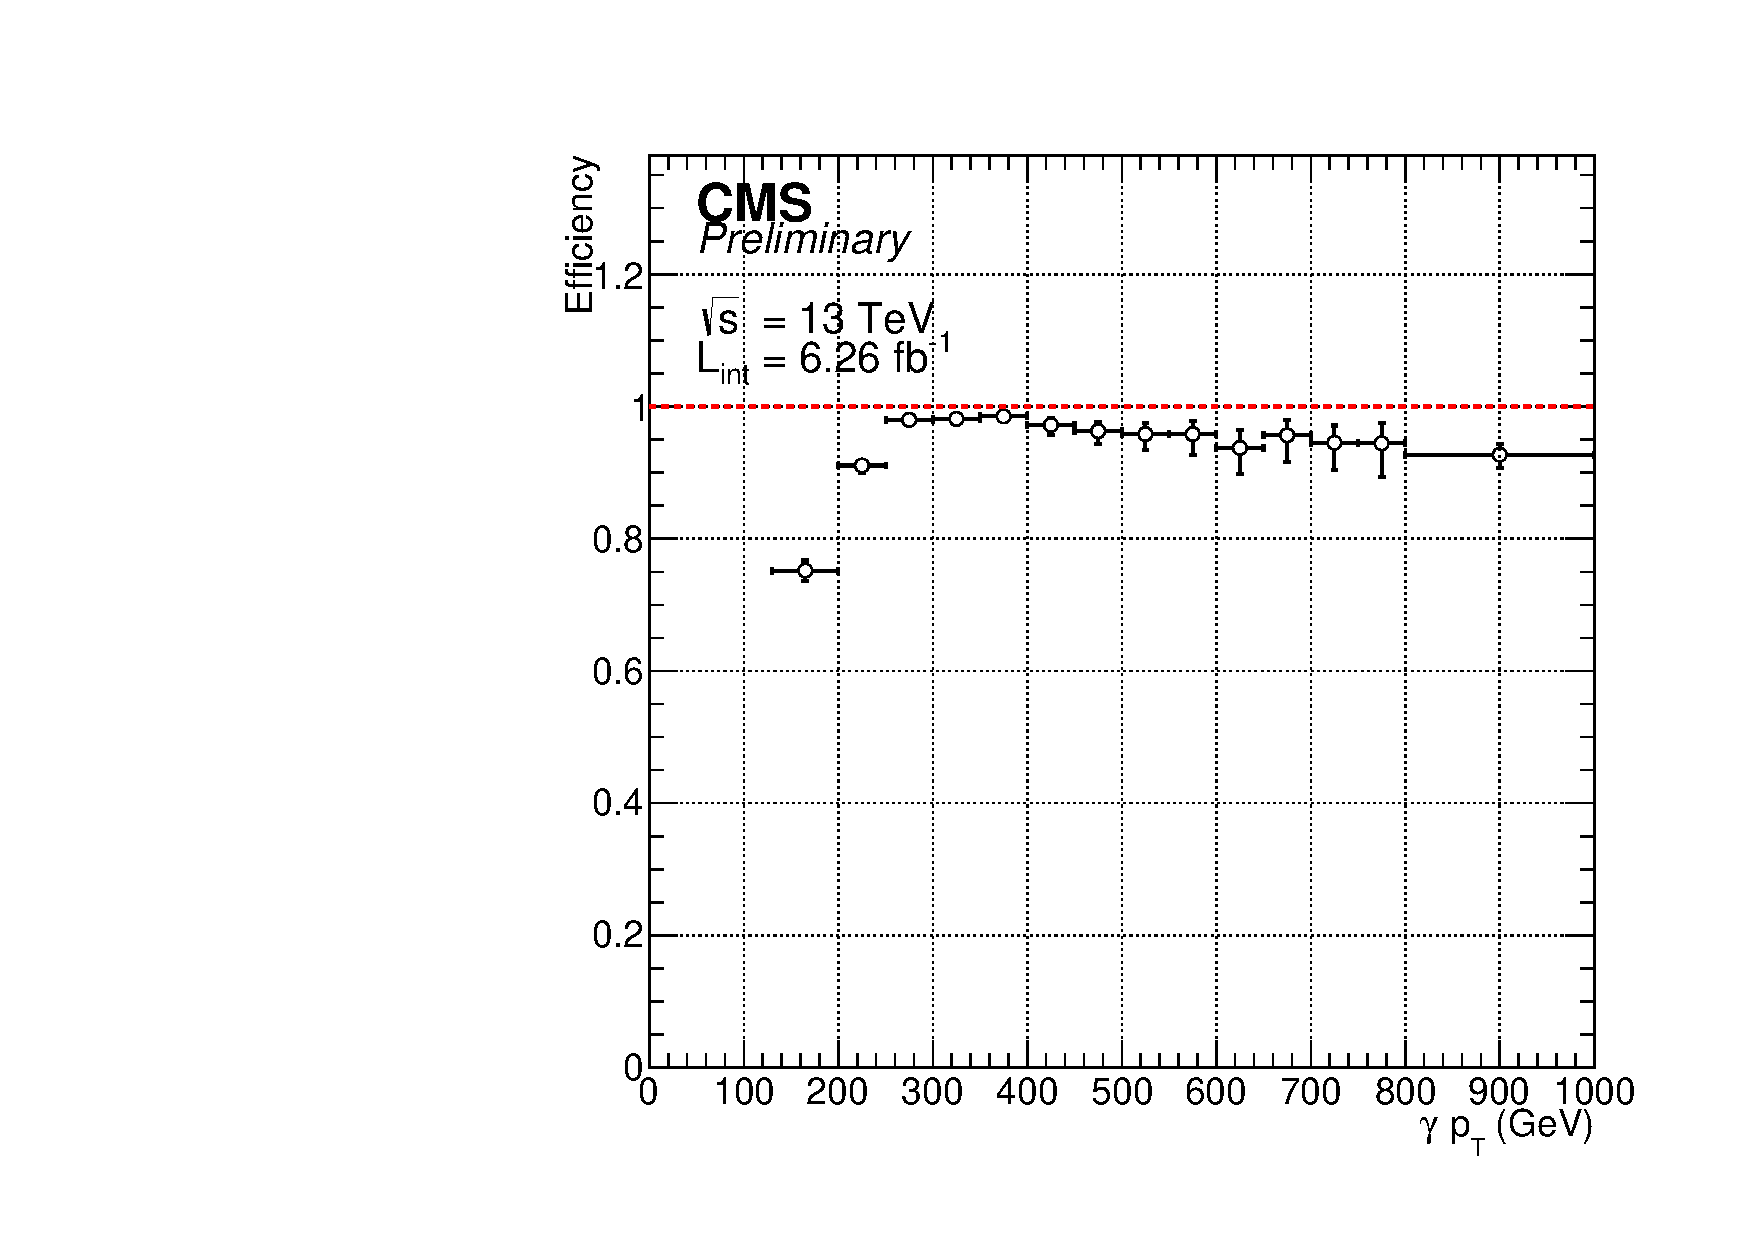
\includegraphics[width=0.4\textwidth]{figures/Trigger/Photon/HLT_Photon175_MoM_all_800to999999_mht}} ~~\
%    \subfigure{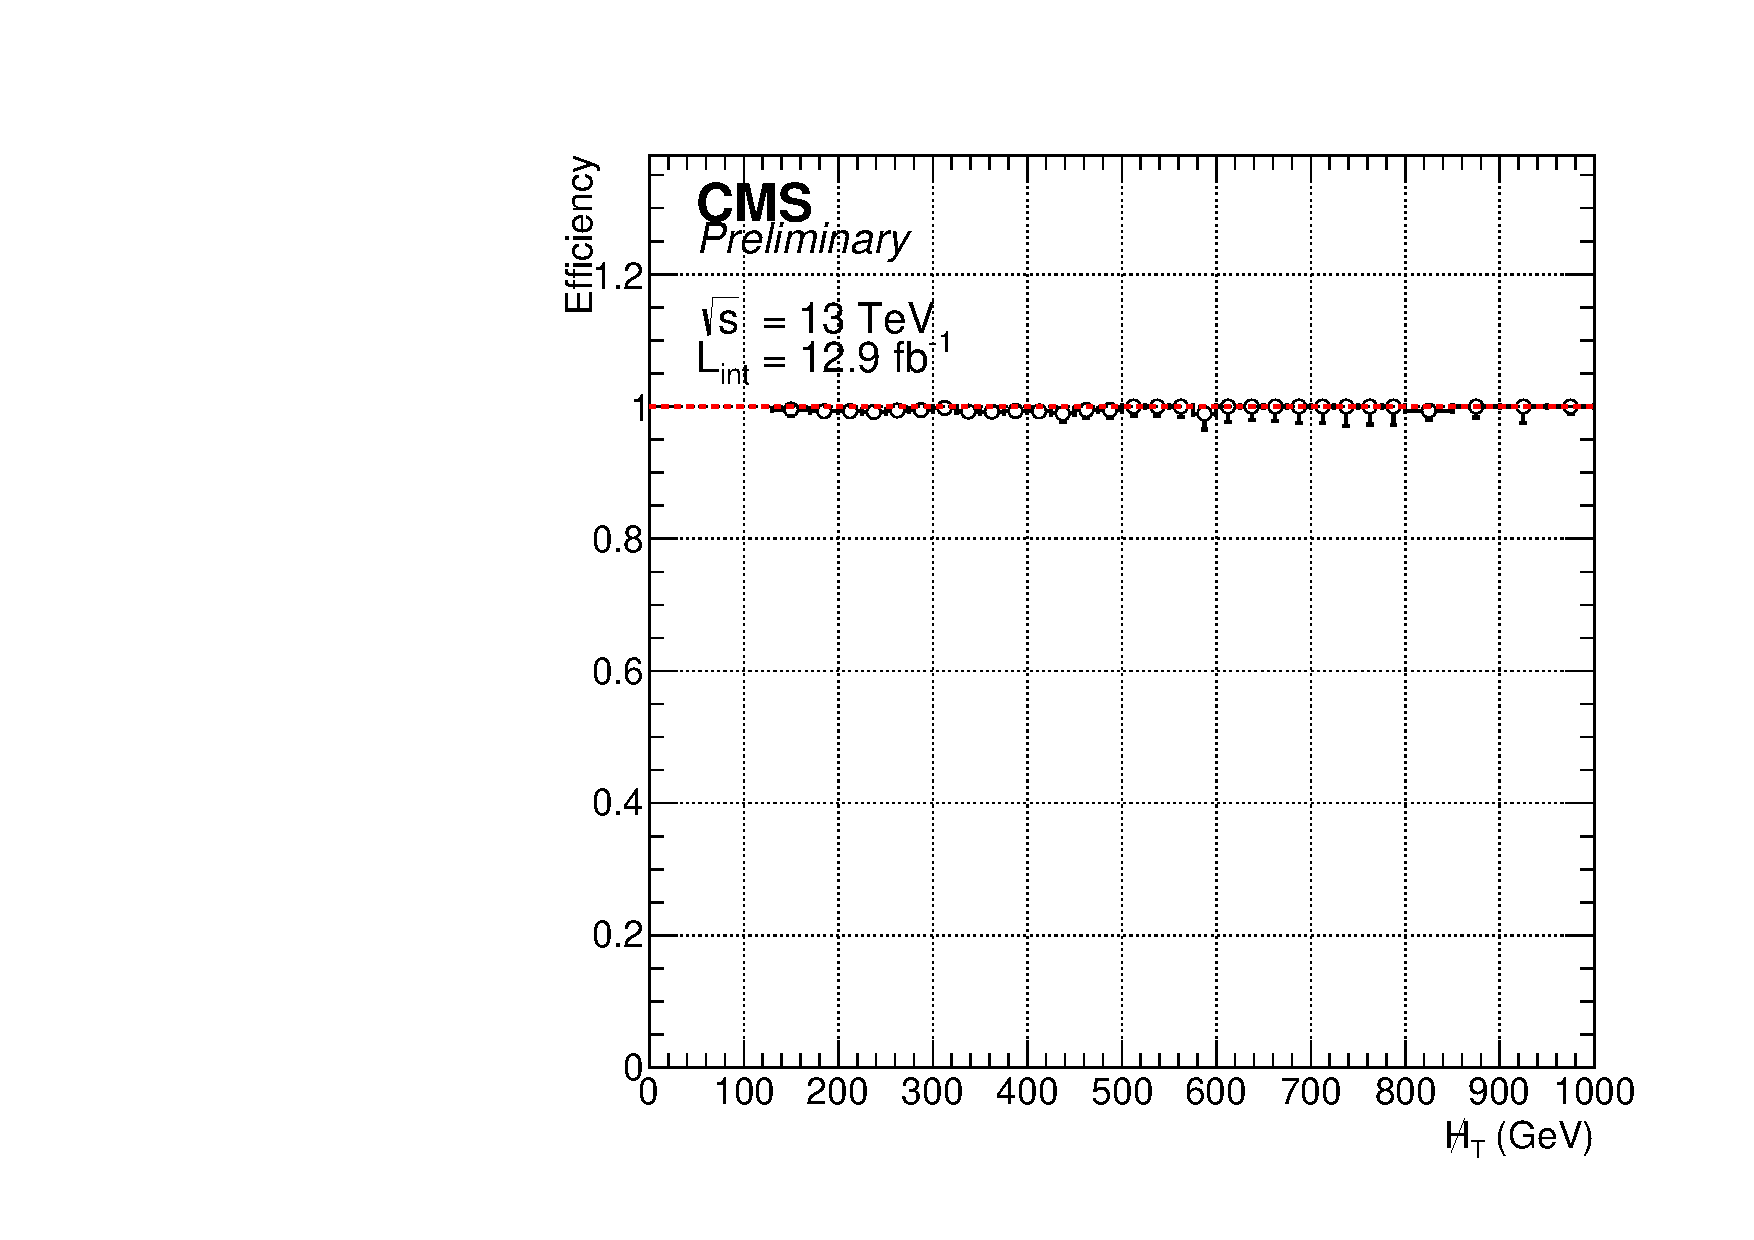
\includegraphics[width=0.4\textwidth]{figures/Trigger/Photon/HLT_PhotonECALHT800_MoM_all_800to999999_mht}} \\
%    \caption{Trigger efficiency as a function of \mht for Photon175
%    (left) and Photon175 OR ECALHT800 (right), measured with events
%    in the JetHT data set passing the \gj control region
%    selection. These are shown inclusive over \scalht (top) and for
%    $\scalht > 800$~GeV (bottom).} 
%    \label{fig:photon_turnons_mht}
%  \end{center}
%\end{figure}

%%____________________________________________________________________________||
